%%%TO-DO
% Literarual review, add more
% why not other methods
% more details in frc forecasting
%change the words 


% Template for PLoS
% Version 3.6 Aug 2022
%
% % % % % % % % % % % % % % % % % % % % % %
%
% -- IMPORTANT NOTE
%
% This template contains comments intended 
% to minimize problems and delays during our production 
% process. Please follow the template instructions
% whenever possible.
%
% % % % % % % % % % % % % % % % % % % % % % % 
%
% Once your paper is accepted for publication, 
% PLEASE REMOVE ALL TRACKED CHANGES in this file 
% and leave only the final text of your manuscript. 
% PLOS recommends the use of latexdiff to track changes during review, as this will help to maintain a clean tex file.
% Visit https://www.ctan.org/pkg/latexdiff?lang=en for info or contact us at latex@plos.org.
%
%
% There are no restrictions on package use within the LaTeX files except that no packages listed in the template may be deleted.
%
% Please do not include colors or graphics in the text.
%
% The manuscript LaTeX source should be contained within a single file (do not use \input, \externaldocument, or similar commands).
%
% % % % % % % % % % % % % % % % % % % % % % %
%
% -- FIGURES AND TABLES
%
% Please include tables/figure captions directly after the paragraph where they are first cited in the text.
%
% DO NOT INCLUDE GRAPHICS IN YOUR MANUSCRIPT
% - Figures should be uploaded separately from your manuscript file. 
% - Figures generated using LaTeX should be extracted and removed from the PDF before submission. 
% - Figures containing multiple panels/subfigures must be combined into one image file before submission.
% For figure citations, please use "Fig" instead of "Figure".
% See http://journals.plos.org/plosone/s/figures for PLOS figure guidelines.
%
% Tables should be cell-based and may not contain:
% - spacing/line breaks within cells to alter layout or alignment
% - do not nest tabular environments (no tabular environments within tabular environments)
% - no graphics or colored text (cell background color/shading OK)
% See http://journals.plos.org/plosone/s/tables for table guidelines.
%
% For tables that exceed the width of the text column, use the adjustwidth environment as illustrated in the example table in text below.
%
% % % % % % % % % % % % % % % % % % % % % % % %
%
% -- EQUATIONS, MATH SYMBOLS, SUBSCRIPTS, AND SUPERSCRIPTS
%
% IMPORTANT
% Below are a few tips to help format your equations and other special characters according to our specifications. For more tips to help reduce the possibility of formatting errors during conversion, please see our LaTeX guidelines at http://journals.plos.org/plosone/s/latex
%
% For inline equations, please be sure to include all portions of an equation in the math environment.  For example, x$^2$ is incorrect; this should be formatted as $x^2$ (or $\mathrm{x}^2$ if the romanized font is desired).
%
% Do not include text that is not math in the math environment. For example, CO2 should be written as CO\textsubscript{2} instead of CO$_2$.
%
% Please add line breaks to long display equations when possible in order to fit size of the column. 
%
% For inline equations, please do not include punctuation (commas, etc) within the math environment unless this is part of the equation.
%
% When adding superscript or subscripts outside of brackets/braces, please group using {}.  For example, change "[U(D,E,\gamma)]^2" to "{[U(D,E,\gamma)]}^2". 
%
% Do not use \cal for caligraphic font.  Instead, use \mathcal{}
%
% % % % % % % % % % % % % % % % % % % % % % % % 
%
% Please contact latex@plos.org with any questions.
%
% % % % % % % % % % % % % % % % % % % % % % % %

\documentclass[10pt,letterpaper]{article}
\usepackage[top=0.85in,left=2.75in,footskip=0.75in]{geometry}

% amsmath and amssymb packages, useful for mathematical formulas and symbols
\usepackage{amsmath,amssymb}

% Use adjustwidth environment to exceed column width (see example table in text)
\usepackage{changepage}

% textcomp package and marvosym package for additional characters
\usepackage{textcomp,marvosym}

% cite package, to clean up citations in the main text. Do not remove.
\usepackage{cite}

% Use nameref to cite supporting information files (see Supporting Information section for more info)
\usepackage{nameref,hyperref}

% line numbers
\usepackage[right]{lineno}

% ligatures disabled
\usepackage[nopatch=eqnum]{microtype}
\DisableLigatures[f]{encoding = *, family = * }

% color can be used to apply background shading to table cells only
\usepackage[table]{xcolor}

% array package and thick rules for tables
\usepackage{array}

% create "+" rule type for thick vertical lines
\newcolumntype{+}{!{\vrule width 2pt}}

% Command for inserting editorial comments
\newcommand{\roni}[1]{\textcolor{blue}{[Roni Comment: #1]}}

% create \thickcline for thick horizontal lines of variable length
\newlength\savedwidth
\newcommand\thickcline[1]{%
  \noalign{\global\savedwidth\arrayrulewidth\global\arrayrulewidth 2pt}%
  \cline{#1}%
  \noalign{\vskip\arrayrulewidth}%
  \noalign{\global\arrayrulewidth\savedwidth}%
}

% \thickhline command for thick horizontal lines that span the table
\newcommand\thickhline{\noalign{\global\savedwidth\arrayrulewidth\global\arrayrulewidth 2pt}%
\hline
\noalign{\global\arrayrulewidth\savedwidth}}


% Remove comment for double spacing
%\usepackage{setspace} 
%\doublespacing

% Text layout
\raggedright
\setlength{\parindent}{0.5cm}
\textwidth 5.25in 
\textheight 8.75in

% Bold the 'Figure #' in the caption and separate it from the title/caption with a period
% Captions will be left justified
\usepackage[aboveskip=1pt,labelfont=bf,labelsep=period,justification=raggedright,singlelinecheck=off]{caption}
\renewcommand{\figurename}{Fig}

% Use the PLoS provided BiBTeX style
\bibliographystyle{plos2015}

% Remove brackets from numbering in List of References
\makeatletter
\renewcommand{\@biblabel}[1]{\quad#1.}
\makeatother

%Extra Package Added
\usepackage{algpseudocode}
\usepackage{algorithm}
\usepackage{bbm}
\usepackage{makecell}
\usepackage{multirow}
\usepackage{graphicx}


% Header and Footer with logo
\usepackage{lastpage,fancyhdr,graphicx}
\usepackage{epstopdf}
%\pagestyle{myheadings}
\pagestyle{fancy}
\fancyhf{}
%\setlength{\headheight}{27.023pt}
%\lhead{\includegraphics[width=2.0in]{PLOS-submission.eps}}
\rfoot{\thepage/\pageref{LastPage}}
\renewcommand{\headrulewidth}{0pt}
\renewcommand{\footrule}{\hrule height 2pt \vspace{2mm}}
\fancyheadoffset[L]{2.25in}
\fancyfootoffset[L]{2.25in}
\lfoot{\today}

%% Include all macros below

\newcommand{\lorem}{{\bf LOREM}}
\newcommand{\ipsum}{{\bf IPSUM}}

%% END MACROS SECTION


\begin{document}
\vspace*{0.2in}

% Title must be 250 characters or less.
\begin{flushleft}
{\Large
\textbf\newline{Real-time Forecasting of Data Revisions in Epidemic Surveillance Streams} % Please use "sentence case" for title and headings (capitalize only the first word in a title (or heading), the first word in a subtitle (or subheading), and any proper nouns).
}
\newline
% Insert author names, affiliations and corresponding author email (do not include titles, positions, or degrees).
\\
Jingjing Tang\textsuperscript{1*},
Aaron Rumack\textsuperscript{2},
Bryan Wilder\textsuperscript{2},
Roni Rosenfeld\textsuperscript{2},
\\
\bigskip
\textbf{1} Computational Biology Department, Carnegie Mellon University, Pittsburgh, PA, USA
\\
\textbf{2} Machine Learning Department, Carnegie Mellon University, Pittsburgh, PA, USA
\\
\bigskip

% Use the asterisk to denote corresponding authorship and provide email address in note below.
*Corresponding author, jtang2@andrew.cmu.edu

\end{flushleft}
% Please keep the abstract below 300 words
\section*{Abstract}
Epidemic data streams undergo frequent revisions due to reporting delays ("backfill") and other factors. Relying on tentative surveillance values can seriously degrade the quality of situational awareness, forecasting accuracy and decision-making. We introduce Delphi Revision Forecast (Delphi-RF), a real-time data revision forecasting\footnote{We use the term “data revision forecasting” to refer to the problem of predicting current quantities based solely on their preliminary measurements.
We reserve the term “nowcasting” to refer to the more general problem of predicting current quantities based on any data available currently, including other data sources.} framework using nonparametric quantile regression, applicable to both counts and proportions (fractions) in public health reporting. By incorporating all available revisions up to a given observation date, Delphi-RF models revision dynamics and generates distributional forecasts of finalized surveillance values. Applied to daily COVID-19 data (insurance claims, antigen tests, confirmed cases) and weekly dengue and influenza-like illness (ILI) case counts, Delphi-RF delivers accurate revision forecasts, particularly in early reporting stages. In addition, it improves computational efficiency by more than tenfold over existing methods, making it a scalable solution for real-time public health surveillance.


% Please keep the Author Summary between 150 and 200 words
% Use first person. PLOS ONE authors please skip this step. 
% Author Summary not valid for PLOS ONE submissions.   
\section*{Author summary}
Accurate and reliable forecasts of infectious disease epidemics, such as COVID-19, are essential but challenging. The presence of data revisions in public health data streams can introduce significant bias in both predictors and responses, leading to suboptimal situational awareness, preparedness, and downstream countermeasure design. To address this issue, we propose a modeling framework that leverages historical revision patterns to generate distributional forecasts of finalized surveillance values. Applicable to both count-type and fraction-type data across various temporal resolutions and epidemic surveillance data streams, our approach ensures real-time accuracy, even with only early revisions available. Moreover, our method achieves competitive or superior forecast accuracy compared to existing methods, while also demonstrating a 10-100x improvement in computational efficiency.
\linenumbers

% Use "Eq" instead of "Equation" for equation citations.
\section{Introduction}

# add van2019nowcasting
The COVID-19 pandemic, as a global public health crisis, has precipitated unprecedented societal, economic, and political disruptions, underscoring the imperative of real-time epidemic forecasting. However, many of the epidemic surveillance values published by public health surveillance data systems are often and repeatedly revised in subsequent releases after their first release, and do not accurately reflect disease activity in real time. This often leads to biased and error-prone situational awareness\cite{McGough2020}\cite{Rosenfeld2021} and poses substantial hurdles to achieving real-time epidemic forecast accuracy.

The impact of reporting delays and subsequent data revisions has been discussed not only in the context of public health studies: from influenza\cite{chakraborty2018know} to dengue \cite{rangarajan2019forecasting} to COVID-19 forecasting\cite{rodriguez2021deepcovid}\cite{adiga2020mathematical}, but also in the macroeconomic domain\cite{clements2019data}. Data revisions arise from various factors, including error corrections, infrastructure limitations, and varying delays between data collection and reporting\cite{reich2019collaborative}\cite{Chakraborty2018}. These factors affect surveillance values differently, leading to distinct data revision patterns. For example, case counts typically increase monotonically during the revision process, a phenomenon commonly referred to as "backfill.". However, epidemic fractions (e.g., the percentage of positive COVID-19 insurance claims out of total claims) often fluctuate—either increasing or decreasing—dramatically due to different backfill dynamics of the numerator and denominator.

Several studies have sought to address these issues, focusing mainly on seasonal infectious diseases with years of weekly historical data. For example, Bastos et al. (2019) developed a Bayesian framework utilizing the Laplace approximation (INLA), applying it to weekly dengue data from Rio de Janeiro and weekly SARI data from Paraná, Brazil \cite{bastos2019modelling}. Chakraborty et al. (2014) used a linear regression algorithm to adjust provisional surveillance data for influenza-like illness (ILI) case counts forecasting across 15 Latin American countries \cite{chakraborty2014forecasting}. Brooks et al. (2018) estimated the distribution of revised updates for influenza data using the residual density method, focusing on weekly ILI data \cite{brooks2018nonmechanistic}. Osthus et al. (2019) proposed a forecaster that accounts for backfill uncertainty but does not explicitly model its effects \cite{osthus2019even}. McGough et al. (2020) introduced the Nowcasting by Bayesian Smoothing (NobBS) framework, a flexible generalized Bayesian model for dengue and influenza case counts that improves uncertainty estimation and accommodates temporal variation in delay probabilities \cite{McGough2020}. Stoner et al. (2020) proposed a generalized Dirichlet-multinomial mixture framework, modeling total case counts and multinomial probabilities with temporally varying parameters, which was applied to weekly dengue fever cases in Rio de Janeiro \cite{stoner2020multivariate}.

Comparatively, while COVID-19 surveillance data offer finer temporal granularity by transitioning from weekly to daily updates, this increased frequency introduces substantial noise, making it challenging to obtain stable values for features that capture revision patterns. To address these challenges, Kamarthi et al. (2021) developed a neural network-based framework to refine COVID-19 forecasts using weekly case count data \cite{kamarthi2021back2future}. While this approach leverages modern computational techniques, it requires substantial computing resources and does not account for the statistical properties of public health datasets. Kline et al. (2022) proposed a Bayesian spatiotemporal nowcasting model to estimate COVID-19 case counts at the county level in Ohio, incorporating an autoregressive structure to capture temporal dynamics \cite{kline2022bayesian}. Both methods focus exclusively on count-type data, and were evaluated only for the pre-Delta period. Among existing methods, Epinowcast\cite{epinowcast} stands out as a strong competitor, leveraging a full Bayesian framework for nowcasting with robust uncertainty quantification. However, Bayesian inference is computationally intensive, often requiring long runtimes, which can limit real-time applicability. Moreover, Bayesian models like Epinowcast primarily operate on count-type data and are less adaptable to fraction-based signals. Many important public health indicators—including antigen test positivity rates, hospitalization ratios, and syndromic surveillance measures—are represented as fractions rather than raw counts. This limitation arises because Bayesian methods typically assume an underlying mechanistic process governing count evolution, whereas fraction-type signals often lack a well-defined generative model. 
 
In the broader field of forecasting, Croushore (2006, 2011) surveyed data revisions and real-time analysis in macroeconomics, while Clements (2019) summarized data revisions modeling approaches, including state-space models \cite{croushore2006forecasting} \cite{croushore2011forecasting} \cite{clements2019data}. However, these macroeconomic approaches are not directly transferable to public health data.

In this paper, we focus on the distributional forecasting of finalized surveillance values in \textit{real time}. We introduce Delphi-Revision Forecasting (Delphi-RF), a robust and operational framework for correcting data revisions, which is openly available at https://github.com/cmu-delphi/DelphiRF. Delphi-RF is designed to handle signals with varying temporal resolutions and is applicable to both count-based and fraction-based data. When estimating quantities relative to a given observation date $s$, our approach ensures that only data available up to that date are used. Specifically, the correction system uses all revisions recorded up to $s$ to estimate the probability distribution of the finalized values, which become fully available only at a later stage.

The Delphi Group at Carnegie Mellon University curates real time infectious disease indicators and makes them accessible via public API\cite{reinhart2021open}.  When applied to a variety of such indicators, we have shown that Delphi-RF provides competitive or superior forecast accuracy for data revisions, including for COVID-19, dengue fever, and influenza-like illness (ILI). Moreover, Delphi-RF achieves an improvement of over an order of magnitude (10x) in computational efficiency compared to existing methods, making it a scalable and practical solution for real-time public health surveillance.

The remainder of this paper is organized as follows. Section 2 introduces the problem setup along with key terminology and notation. Section 3 provides a detailed description of the model, the evaluation methodology, and the adaptive modeling protocol. In Section 4, we describe the datasets used, the data preprocessing steps, the experimental setup, and the results. This includes the performance of the model on multiple COVID-19 indicators, as well as comparisons with alternative methods applied to different infectious diseases. Finally, Section 5 concludes the paper with a discussion of the findings and an outline of directions for future research.

\begin{figure}[h!]
    \centering
    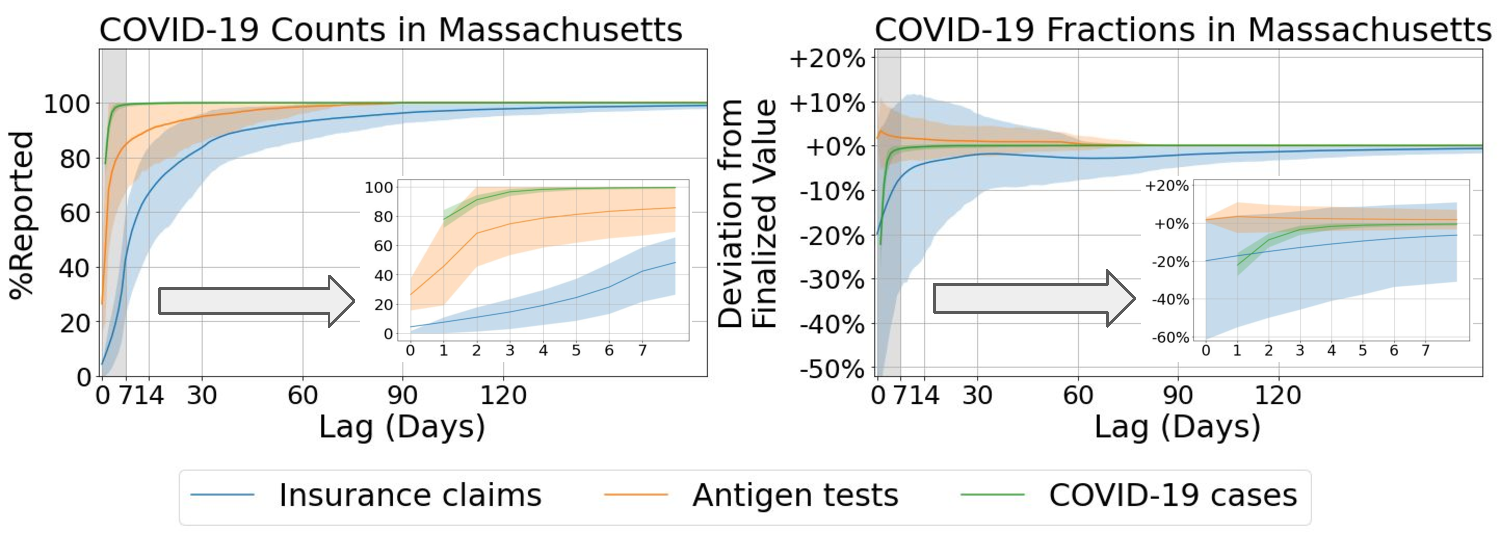
\includegraphics[width=\textwidth]{figs/Intro_fig.pdf}
    \caption{\textit{\textbf{Data revision for different indicators.} Left: Mean percentage of total counts reported, averaged over all reference dates considered, over lags for states in US. The shaded bands correspond to 10\% quantile to 90\% quantile intervals. Right: Mean fraction of COVID-19 fractions normalized by the revised reports 300 days later, averaged over all reference dates considered, over lags for Massachusetts.}}
\end{figure}




\section{Terminology, Notation and Problem Definition}

Throughout this paper, we use the term \emph{reference date} for the date $t$ to which a particular quantity refers, and the term \emph{report date} for the date $s$ in which a particular quantity became available to the model.

Let $Y_{it}$ denote a surveillance value associated with the \emph{reference date} $t$ for location $i$. The time series ${Y_{it}}{t \in T}$ represents the usual uni-variate surveillance data for location $i$, where $T$ denotes a set of reference dates. The value of $Y_{it}$ reported as of date $s$ ($s \ge t$) is denoted by $Y_{itl}$, where $l$ is the \emph{lag}, defined as $l = s - t \in \mathbf{N}$, representing the number of days between the report date $s$ and the reference date $t$. By convention, $l \ge 0$. The value $Y_{itl}$ corresponds to the $(l+1)$th version of $Y_{it}$ (with $l=0$ representing the initial release).

\paragraph{Revision Dynamics:} Due to the existence of data revision, each $Y_{it}$ has its \emph{data revision sequence} $Y_{it}^{t:s}$ as of date $s$, equivalently denoted by $Y_{it,0:(s-t)}$. Only a minimal portion of data revision results from instances where data is initially lost but subsequently recovered, or when data is initially entered incorrectly but corrected later. The predominant share of data revision is usually results from reporting delays. The data revision sequence $Y_{itl}$ tends to asymptote as $l$ approaches a sufficiently large value $L_{it}$. We call $L_{it}$ the \emph{target lag}, and $Y_{itL_{it}}$ is called the target value of $Y_{it}$. 

To reduce confusion, $Y_{itl}$ represents the most up-to-date version of $Y_{it}$ as of date $s = t+l$ regardless of whether a revision or a report action occurred on date $s$.  It is important to distinguish between \emph{no reported revision} and \emph{a report of no revision}. In cases where a revision occurs but is not reported, this scenario is categorized as no reported revision. In this paper, we pragmatically assume that no reported revision is equivalent to a report of no revision, as the distinction is not recorded in the data available to us. Namely, when there is no report for $Y_{itl}$, we define 
$$
    Y_{itl}=
\begin{cases}
    0,           & \text{if } l = 0\\
    Y_{it(l-1)}, & \text{if } l\geq 1\\    
\end{cases}
$$
We then uniformly refer to $Y_{itl}$ as the $(l+1)$th release (or the $l$th revision) of $Y_{it}$.

% We refer to $Y_{it}=Y_{it\infty}$ as the \emph{finalized} surveillance value.
%% Roni: Y_}it\infty} is a problematic concept, because the reporting sequence is always finite.  Above we defined "finalized value" as Y_{itL}.
%% Jingjing: Later on, we decided to give up the term "finalized" to reduce confusion.

\paragraph{Problem Setup:}
In practice, the time required for the convergence of the revision exhibits considerable variability across different data streams, locations $i$ and reference dates $t$, and can be exceptionally large. Figure S1 (in the Appendix) provides an illustration in which, for COVID-19 claims reports with a reference date of 2021-08-01, most states require more than 180 days (approximately half a year) for the data revision sequences to converge. 

However, such values of \( L_{it} \) are not available in real-time since it is impossible to determine whether the revision for \( Y_{it} \) has been finalized. This creates a challenge in selecting the target value corresponding to a target horizon \( L_{it} \) for \( Y_{it} \). On one hand, we prefer a long target horizon to ensure that the reporting sequence has asymptoted or is close to asymptoting. We aim for greater accuracy, which means that we tend to select a target lag \( L_{it} \) that is large enough to ensure that the estimates closely approximate the value to which \( Y_{it} \) asymptotes. On the other hand, we want our model to remain adaptive. Data revision dynamics evolve over time, and training on outdated data could result in model mismatch or bias. Selecting a larger lag \( L_{it} \) limits the model to data from \( L_{it} \) days ago, whereas a smaller lag allows the model to respond more effectively to recent changes in the data.

The selection of the target lag involves a trade-off between accuracy and adaptability. To address this, we choose a fixed target lag \( L \) for all reference dates and locations that captures the majority of revisions (e.g., 90\% of case counts reported) after exploring the available revision history of a public health data stream. Additionally, we ensure that the target lag does not exceed 60 days to maintain the model's adaptability.

Given a revision sequence $Y_{it, 0:l}$, our goal is to provide a distributional estimate of the target $Y_{itL}$ for a suitably large $L$ in the form of a set of quantile estimates $Q_{Y_{itL}}^{\tau}$ for a pre-determined set of quantiles $\tau$s. 









\section{Methods}
In this section, we introduce a non-parametric model, Delphi Revision Forecast (Delphi-RF), which leverages quantile regression to characterize the dynamics of data revisions. Let $L$ denote the target lag. For a random variable $Y_{itl}$ representing the value for location $i$ and reference date $t$, as reported at time $t + l$, the corresponding target is $Y_{itL}$. We denote the cumulative distribution function of $Y_{itL}$ as
\[
F_{Y_{itL}}(y) = P(Y_{itL} \leq y).
\]
The $\tau$th quantile of $Y_{itL}$ is defined as
\[
Q_{Y_{itL}}^{\tau} = \inf \left\{ y : F_{Y_{itL}}(y) \geq \tau \right\}, \quad \tau \in (0, 1).
\]

Given the potential nonlinear effects of calendar factors such as day-of-week and week-of-month, and motivated by the objective of minimizing relative error between estimates and targets, we adopt a multiplicative model to estimate the conditional quantiles of the log-transformed target. To avoid undefined values when reported counts are zero, we apply a natural logarithmic transformation, defined as $f(x) = \log(x + 1)$, to all relevant quantities. Since $f(\cdot)$ is a monotonically increasing function, the quantile of the transformed target equals the transformed quantile of the target:
\[
Q_{f(Y_{itL})}^{\tau} = f\left(Q_{Y_{itL}}^{\tau}\right).
\]

At any given estimation date (a report date) $s_0$, our goal is to make distributional estimates of $Y_{itL}$ for all reference date $t \in (s_0-L, s_0]$ based on data that is available as of date $s_0$. To simplify notation, we use $f(Y_{itL})|X_{itl}$ to represent $f(Y_{itL})$ as conditioned on the feature vector $X_{itl}$, which is based on $\{Y_{itl}\}_{t+l \leq s_0, l\in [0, L)}$. Therefore, our model is 
\begin{align*} 
Q_{f(Y_{itL})|X_{itl}}^{\tau} &=  X_{itl}\beta^{\tau}
\end{align*}

We incorporate features to account for week-of-month effects based on report dates, as well as day-of-week effects based on both report dates and reference dates. To capture week-of-month effects, we use the indicator \( \mathbf{I}_{\text{first-week}(t)} \), which identifies whether a given date \( t \) falls within the first week of a month, where each week begins on a Sunday. If date \( t \) corresponds to the final days of a month and overlaps both the fifth week of the current month and the first week of the subsequent month, it is still classified as part of the first week. For day-of-week effects, we define the vector \( \mathbf{e}_{wd(t)} \) as a one-hot encoded vector, where the first element is set to 0 if \( t \) is a Monday, 1 if \( t \) falls on a weekend, and 2 otherwise. To ensure model identifiability, we omit one category from each of the two one-hot encoded feature sets.

We incorporate two features to represent disease activity levels.  The first one is the 7day moving average of the current reports. Let \( \widetilde{Y}_{itl} \) denote the 7-day moving average of values reported with report date \( t + l \), defined as

\[
\widetilde{Y}_{itl} = \sum_{v=0}^{6} Y_{i(t - v)(l + v)}.
\] 
Given the significant skewness in \( Y_{itl} \), we apply a square root transformation to improve linearity between the quantiles and the transformed variable. We then construct a one-hot encoded vector \( \mathbf{e}_{\sqrt{\widetilde{Y}_{itl}}} \), whose components correspond to four equal-width bins of \( \sqrt{\widetilde{Y}_{itl}} \), determined based on its empirical distribution in the training data. To ensure identifiability, only three of the four indicator variables are included in the model. In practice, to mitigate instability arising from sparsely populated bins—particularly in the distributional tails—rare categories are merged into the reference bin, promoting stable estimation while preserving model identifiability.

To capture changes in revision patterns, we introduce two extra set of features: 
1) $f(\widetilde{Y}_{i(t-1)(l+1)}, f(\widetilde{Y}_{i(t-7)(l+7)} $ which are the most recent revision for the reference date 1 day and 7 days ago, which can provide extra information about how the epidemic trend changes in the near history; 2)  $(f(\widetilde{Y}_{i(t-1)(l+1)} - f(\widetilde{Y}_{i(t-1)l_{\text{min}}}), (f(\widetilde{Y}_{i(t-7)(l+7)} - f(\widetilde{Y}_{i(t-7)l_{\text{min}}})$ how much the revision is made in the latest release for the reference date $t-1$ and $t-7$ compared to their first release.  Such a design considering the exact value of the most recent revisions and how much the revision is made compared to the first release is for Reduces noise, improve numerical stability, since the first release are usually small and noisy.

To capture changes in revision patterns, we introduce two additional sets of features. The first consists of the most recent revisions for the reference dates \( t - 1 \) and \( t - 7 \), defined as \( f(\widetilde{Y}_{i(t-1)(l+1)}) \) and \( f(\widetilde{Y}_{i(t-7)(l+7)}) \), which provide information on short-term epidemic trends. The second set measures the magnitude of revision for these same reference dates relative to their initial releases, given by \( f(\widetilde{Y}_{i(t-1)(l+1)}) - f(\widetilde{Y}_{i(t-1)l_{\text{min}}}) \) and \( f(\widetilde{Y}_{i(t-7)(l+7)}) - f(\widetilde{Y}_{i(t-7)l_{\text{min}}}) \). This design captures both the current epidemic intensity and the magnitude of revisions relative to the first report, offering insight into how strongly early reports are updated across different levels of disease activity. It also enhances numerical stability, as initial releases are typically small and highly variable.

Now, the full model can be expressed as:

\begin{align*} 
 &Q_{f(Y_{itL})|X_{itl}}^{\tau} \\
= &X_{itl} \beta^{\tau} \\
= &\beta_0^{\tau} + \mathbf{I}_{\text{first-week}(t+l)} \beta_1^{\tau} 
&& \text{(Intercept, week-of-month effect)} \\
& + \mathbf{e}_{wd(t)} \beta_{2:3}^{\tau} + \mathbf{e}_{wd(t+l)} \beta_{4:5}^{\tau}
&& \text{(Day-of-week effects)} \\
& + f(\widetilde{Y}_{itl}) \beta_6^{\tau} + \mathbf{e}_{\sqrt{\widetilde{Y}_{itl}}} \beta_{7:9}^{\tau}
&& \text{(Disease activity level)} \\
&+ \left(f(\widetilde{Y}_{i(t-1)(l+1)}) - f(\widetilde{Y}_{i(t-1)l_{\text{min}}})\right) \beta_{10}^{\tau}
&& \text{(Recent revision magnitude, \(t{-}1\))} \\
&+ \left(f(\widetilde{Y}_{i(t-7)(l+7)}) - f(\widetilde{Y}_{i(t-7)l_{\text{min}}})\right) \beta_{11}^{\tau}
&& \text{(Recent revision magnitude, \(t{-}7\))} \\
& + f(\widetilde{Y}_{i(t-1)(l+1)}) \beta_{12}^{\tau} + f(\widetilde{Y}_{i(t-7)(l+7)}) \beta_{13}^{\tau}
&& \text{(Short-term epidemic trends)}\\
\end{align*}

We estimate the coefficients by solving the following regularized quantile regression problem:
\[
\beta^{\tau} = \arg\min_{\beta} \sum_{t = s_0 - L - W}^{s_0 - L} \sum_{l = \max(l_{\min}, l - c)}^{\min(L - 1, l + c)} w_{itl} \cdot \rho_\tau \left(f(Y_{itL}) - X_{itl} \beta\right) + \lambda \|\beta\|_1.
\]

where \( \rho_\tau(\cdot) \) denotes the quantile loss function \cite{Koenker1978}, and \( \|\cdot\|_1 \) is the \( \ell_1 \)-norm.
 
The flexibility and adaptability of this framework are governed by four key hyperparameters, each influencing a different dimension of the training procedure. These hyperparameters determine how data are selected, weighted, and regularized during model estimation:

\begin{enumerate}
    \item \textbf{Regularization strength} ($\lambda$): An $\ell_1$ (Lasso) penalty is applied to the coefficient vector to promote sparsity in the model, thereby reducing overfitting and enhancing interpretability. The hyperparameter $\lambda$ controls the strength of this regularization and governs the trade-off between model complexity and fit.

    \item \textbf{Training window length} ($W$): Instead of using the entire historical dataset, we restrict training to the most recent $W$ days for which the target is available prior to the evaluation time. This temporal constraint ensures that the model focuses on recent reporting behavior while still incorporating sufficient historical information for effective training.
    
    \item \textbf{Lag padding} ($c$): Because data revision patterns vary substantially across reporting lags, we modify the regularized data revision correction framework by narrowing the lag window and training separate models for quantities reported at different lags. In theory, this is equivalent to fitting a single generalized linear model to the pooled dataset. However, this equivalence breaks down under $\ell_1$ regularization, as the lasso alters the solution space by favoring sparsity and reducing sensitivity to outliers.
    
    To estimate the quantities reported at lag $l$, we define the training set over a local neighborhood of lags, $\mathcal{L}(l, c) = \{l': l - c \leq l' \leq l + c\}$, where $c$ controls the width of the lag window. When $c > 0$, the inverse lag feature ($1/(l+1)$ ) is included to reflect lag-dependent effects across neighboring lags.
    
    Although this strategy requires fitting multiple models and incurs additional computational cost, it improves estimation accuracy by better capturing lag-specific revision dynamics under regularization.    

    \item \textbf{Decay parameter} ($\gamma$): To emphasize training examples that resemble the current epidemic context, we introduce sample-specific weights:
    \[
    w_{itl} = \exp(-\gamma \cdot D^y_{itl} \cdot D^s_{itl}),
    \]
    where $\gamma \geq 0$ controls the sharpness of the weighting scheme. The weight $w_{itl}$ is computed based on the product of two similarity measures, evaluated relative to the estimation date $s_0$:
    \begin{itemize}
        \item $D^y_{itl} = \left|f(\widetilde{Y}_{i(s_0 - l) l}) - f(\widetilde{Y}_{itl})\right|$ quantifies the difference in activity levels between the current observation and the most recent report at lag $l$, measured on the log scale.
        \item $D^s_{itl} = \left|[f(\widetilde{Y}_{i(s_0 - l) l}) - f(\widetilde{Y}_{i(s_0 - l - 7)(l + 7)})] - [f(\widetilde{Y}_{itl}) - f(\widetilde{Y}_{i(t - 7)(l + 7)})]\right|$ captures the difference in 7-day trends between the two time points.
    \end{itemize}
    Larger values of $\gamma$ place greater emphasis on samples with similar epidemic behavior, allowing the model to focus on training points most representative of current conditions.
    
\end{enumerate}


\subsection{Evaluation Metrics}
We use the Weighted Interval Score (WIS) \cite{gneiting2007strictly}, a standard metric for evaluating distributional forecasts, to quantify the distance between the forecast distribution $F$ and the target variable $Y$.
$$
    \mbox{WIS}(F, Y) = 2\sum_{\tau}\phi_{\tau}(Y-Q_Y^{\tau})
$$

where $\phi_{\tau}(x) = \tau|x|$ for $x\geq 0$ and $\phi_{\tau}(x) = (1-\tau)|x|$ for $x<0$, which is called the tilted absolute loss\cite{mcdonald2021can}. $Q_Y^{\tau}$ denotes the forecasted $\tau$th quantile of $Y$. Given a certain estimation task of $Y_{it}$ for location $i$ and reference date $t$ based on the quantities of interest that is available on date $t+l$, the WIS score can be written as 
$$
    \mbox{WIS}(F_{f(Y_{itL}|X_{itl})}, f(Y_{itL})) = 2\sum_{\tau}\phi_{\tau}(f(Y_{itL}) - Q_{f(Y_{itL}|X_{itl})}^{\tau})
$$
where the set $\{ Q_{f(Y_{itL})|X_{itl}}^{\tau} \}_{\tau}$ represents the forecast distribution over quantiles for the log-transformed target value $Y_{itL}$, where $Y_{itL}$ denotes the $L$th revision of $Y_{it}$. If only the median is forecasted, the WIS reduces to the absolute error on the log scale:
$$ \text{WIS}_{itl} = |f(Y_{itL}) - Q_{f(Y_{itL})|X_{itl}}^{0.5} |  $$

Since WIS is computed on the log scale, it adopts a symmetric perspective on relative error, ensuring scale invariance and robustness to variation in magnitude across different reference dates and locations. However, when the target value approaches zero, relative errors can become highly volatile, introducing sensitivity into the evaluation metric.

The quantity $\exp(\text{WIS}) - 1$ approximates the absolute percentage error (APE), allowing for an interpretable link between the log-scale WIS and relative error in the original scale. A smaller $\text{WIS}_{itl}$ therefore indicates a smaller relative error between the distributional forecast and the target. When only the median forecast is considered, $\exp(\text{WIS}) - 1$ coincides with the APE if the projected median is greater than or equal to the observed value, but exceeds the APE otherwise. 

It's worth pointing out that due to the introduction of regularization, WIS differs from the penalized quantile regression loss used to train our estimation models. For model evaluation, we aggregate WIS scores by averaging over all reference dates $t$ and locations $i$ while considering log-scale quantities. This approach leverages the geometric mean, which provides a more accurate assessment of positively skewed relative errors.

\subsection{Adaptive Modeling Protocol}

The correction of real-time data revisions involves repeatedly forecasting target values using epidemic quantities observed up to a given estimation date, denoted by $s_0$. At each estimation date, we simulate the real-time setting by training the model using the latest available revisions of past values. Specifically, the model is provided with the following set of inputs for a given location $i$:

{\scriptsize
\[
\begin{array}{lccccccc}
 & Y_{i,s_0,0} & Y_{i,(s_0{-}1),1} & Y_{i,(s_0{-}2),2} & \cdots & Y_{i,(s_0{-}L{+}1),(L{-}1)} & Y_{i,(s_0{-}L),L} &\cdots \\
\text{Reference date:} & s_0 & s_0{-}1 & s_0{-}2 & \cdots & s_0{-}L{+}1 & s_0{-}L &\cdots\\
\text{Revision index:} & 0\textsuperscript{th} & 1\textsuperscript{st} & 2\textsuperscript{nd} & \cdots & (L{-}1)\textsuperscript{th} & L\textsuperscript{th}&\cdots
\end{array}
\]
}

These values represent the most recent revisions of past observations that would have been available at $s_0$. For example, $Y_{i,s_0,0}$ is the initial report for reference date $s_0$, $Y_{i,(s_0{-}1),1}$ is the second revision for reference date $s_0{-}1$, and so on. As the estimation date progresses from $s_0 -1$ to $s_0$, the data revision sequence

$$ Y_{i,(s_0-L),0:L} = \{Y_{i, (s_0-L), 0}, Y_{i, (s_0-L), 1}, Y_{i, (s_0-L), 2}, \dots, Y_{i, (s_0-L), L}\} $$

is newly added to the training set, while the forecast made for the reference date $s_0{-}L$, based on the 0th through $(L{-}1)$th revisions, can now be evaluated since the target has become available. Data for reference dates $t$ such that $s_0{-}L < t \leq s_0$ continue to serve solely as input covariates to generate real-time forecasts, until their corresponding targets become available.


To select hyperparameters $(c, \lambda, \gamma)$, we perform a grid search with 3-fold cross-validation. At each combination of hyperparameter values, the training set is partitioned into three subsets; in each fold, the model is trained on two subsets and validated on the third. The process is repeated so that each subset serves once as the validation set. Validation performance is evaluated using the average WIS across all reference dates, and the hyperparameter configuration that minimizes this score is selected.



\section{Experimental Results}
In this section, we apply the proposed framework to multiple state-level, daily COVID-19 datasets obtained from the Delphi Epidata API \cite{farrow2015delphi}. These datasets differ in source, structure, and update frequency, and each displays distinct revision patterns, posing challenges for direct performance comparisons across models. Each dataset also exhibits a distinct data revision pattern, making direct comparisons of model performance across datasets nontrivial. 

Beyond evaluating the performance of our proposed method, we compare it against established approaches such as Epinowcast and NobBS in terms of both forecast accuracy and computational efficiency for count-type public health data. We further demonstrate the adaptability of our framework by extending it to weekly datasets, including dengue and ILI case counts. 

All data (including properly versioned datasets) and code used in our analysis are publicly available at:
https://github.com/cmu-delphi/data-revisions-forecasting-paper.

\subsection{Description of Datasets}
\paragraph{Insurance Claims:} We use insurance claims data provided by Change Healthcare (CHNG). CHNG aggregates claim data from numerous healthcare providers and payers, and the information provided by CHNG spans more than two thousand of the most populous US counties, covering more than 45\% of the total US population. Our analysis focuses on a time series comprising the aggregate count of claims featuring ICD codes indicative of COVID-19 diagnoses recorded daily within each county. The reference date corresponds to the claim's date of service, while the report date denotes its appearance in the CHNG database, which may vary considerably depending on providers' claim filing times. Sometimes, Delphi receives the initial report release for a reference date on the same day. We produce forecasts for each report date between 2021-06-01 and 2023-01-10 (a total of 589 days including the Delta wave and the Omicron wave of COVID-19). 

\paragraph{Antigen Tests:}
This dataset is provided by Quidel Corporation (Quidel), which supplies devices used by healthcare providers to conduct COVID-19 antigen tests. We construct a time series of the fraction of positive tests using this dataset. The test records indicate the test date (when the test was conducted) and storage date (when the test was logged into Quidel's MyVirena cloud storage system). The test date serves as the reference date, and test records with a storage date preceding the test date or more than 90 days after are excluded. The report date is defined as the date the records are shared with the Delphi Group via a cloud platform. We produce forecasts for all the states and report dates ranging from 2021-05-18 to 2022-12-12 (a total of 574 days). 

\paragraph{COVID-19 Cases in MA:}
The Massachusetts Department of Public Health (MA-DPH) provides a comprehensive revision history of COVID-19 case reporting\cite{mass_dph_archive}. This dataset includes the 7-day moving average of confirmed COVID-19 cases, updated daily from 2021-01-01, until 2022-07-08. After this date, the reporting frequency transitioned to weekly updates, occurring every Thursday. The first release of the report for a reference date \( t \) is usually made on date \( t+1 \). Unlike the other two datasets—whose fractional denominators exhibit noticeable revision sequences similar to their numerators—a distinctive feature of this dataset is that the COVID-19 confirmed cases are typically normalized by population figures that are sufficiently large to render temporal fluctuations negligible relative to the numerators. We used data reported before 2022-07-08, and produced forecasts for report dates ranging from 2021-07-01, to 2022-06-24 (a span of 359 days).

\subsection{Data Processing}
\paragraph{Data Filtering:}
All datasets are filtered based on the specified time period to ensure data quality. For CHNG outpatient insurance claim data and Quidel antigen test data, this filtering process excludes periods affected by prolonged data reporting issues, such as significant declines in report volume over several months. These anomalies, often manifesting as abrupt shifts in the data distribution, are more indicative of data quality issues than of genuine changes in revision patterns. The MA-DPH case data are filtered to include only the period with consistent daily reporting. As shown in Figure 1, over 90\% of the confirmed cases for a given reference date are reported within 7 days. Given this pattern, developing a data revision forecasting model for weekly reports is unnecessary.

\paragraph{Missing data imputation:}
Before incorporating the data into our framework, we address missing values as defined in the preliminaries. Specifically, for the epidemic count of interest $Y_{it}$ associated with location $i$ and reference date $t$, if $Y_{it}$ has never been reported, impute it as having a historical value of zero. If \( Y_{it} \) is missing for a specific report date \( s \) (i.e., \( Y_{it(s-t)} = \text{NA} \)), we impute it using the most recent available value in the revision sequence of \( Y_{it} \) as of report date \( s \).


\subsection{Experimental Setup}
\begin{figure}[h!]
    \centering
    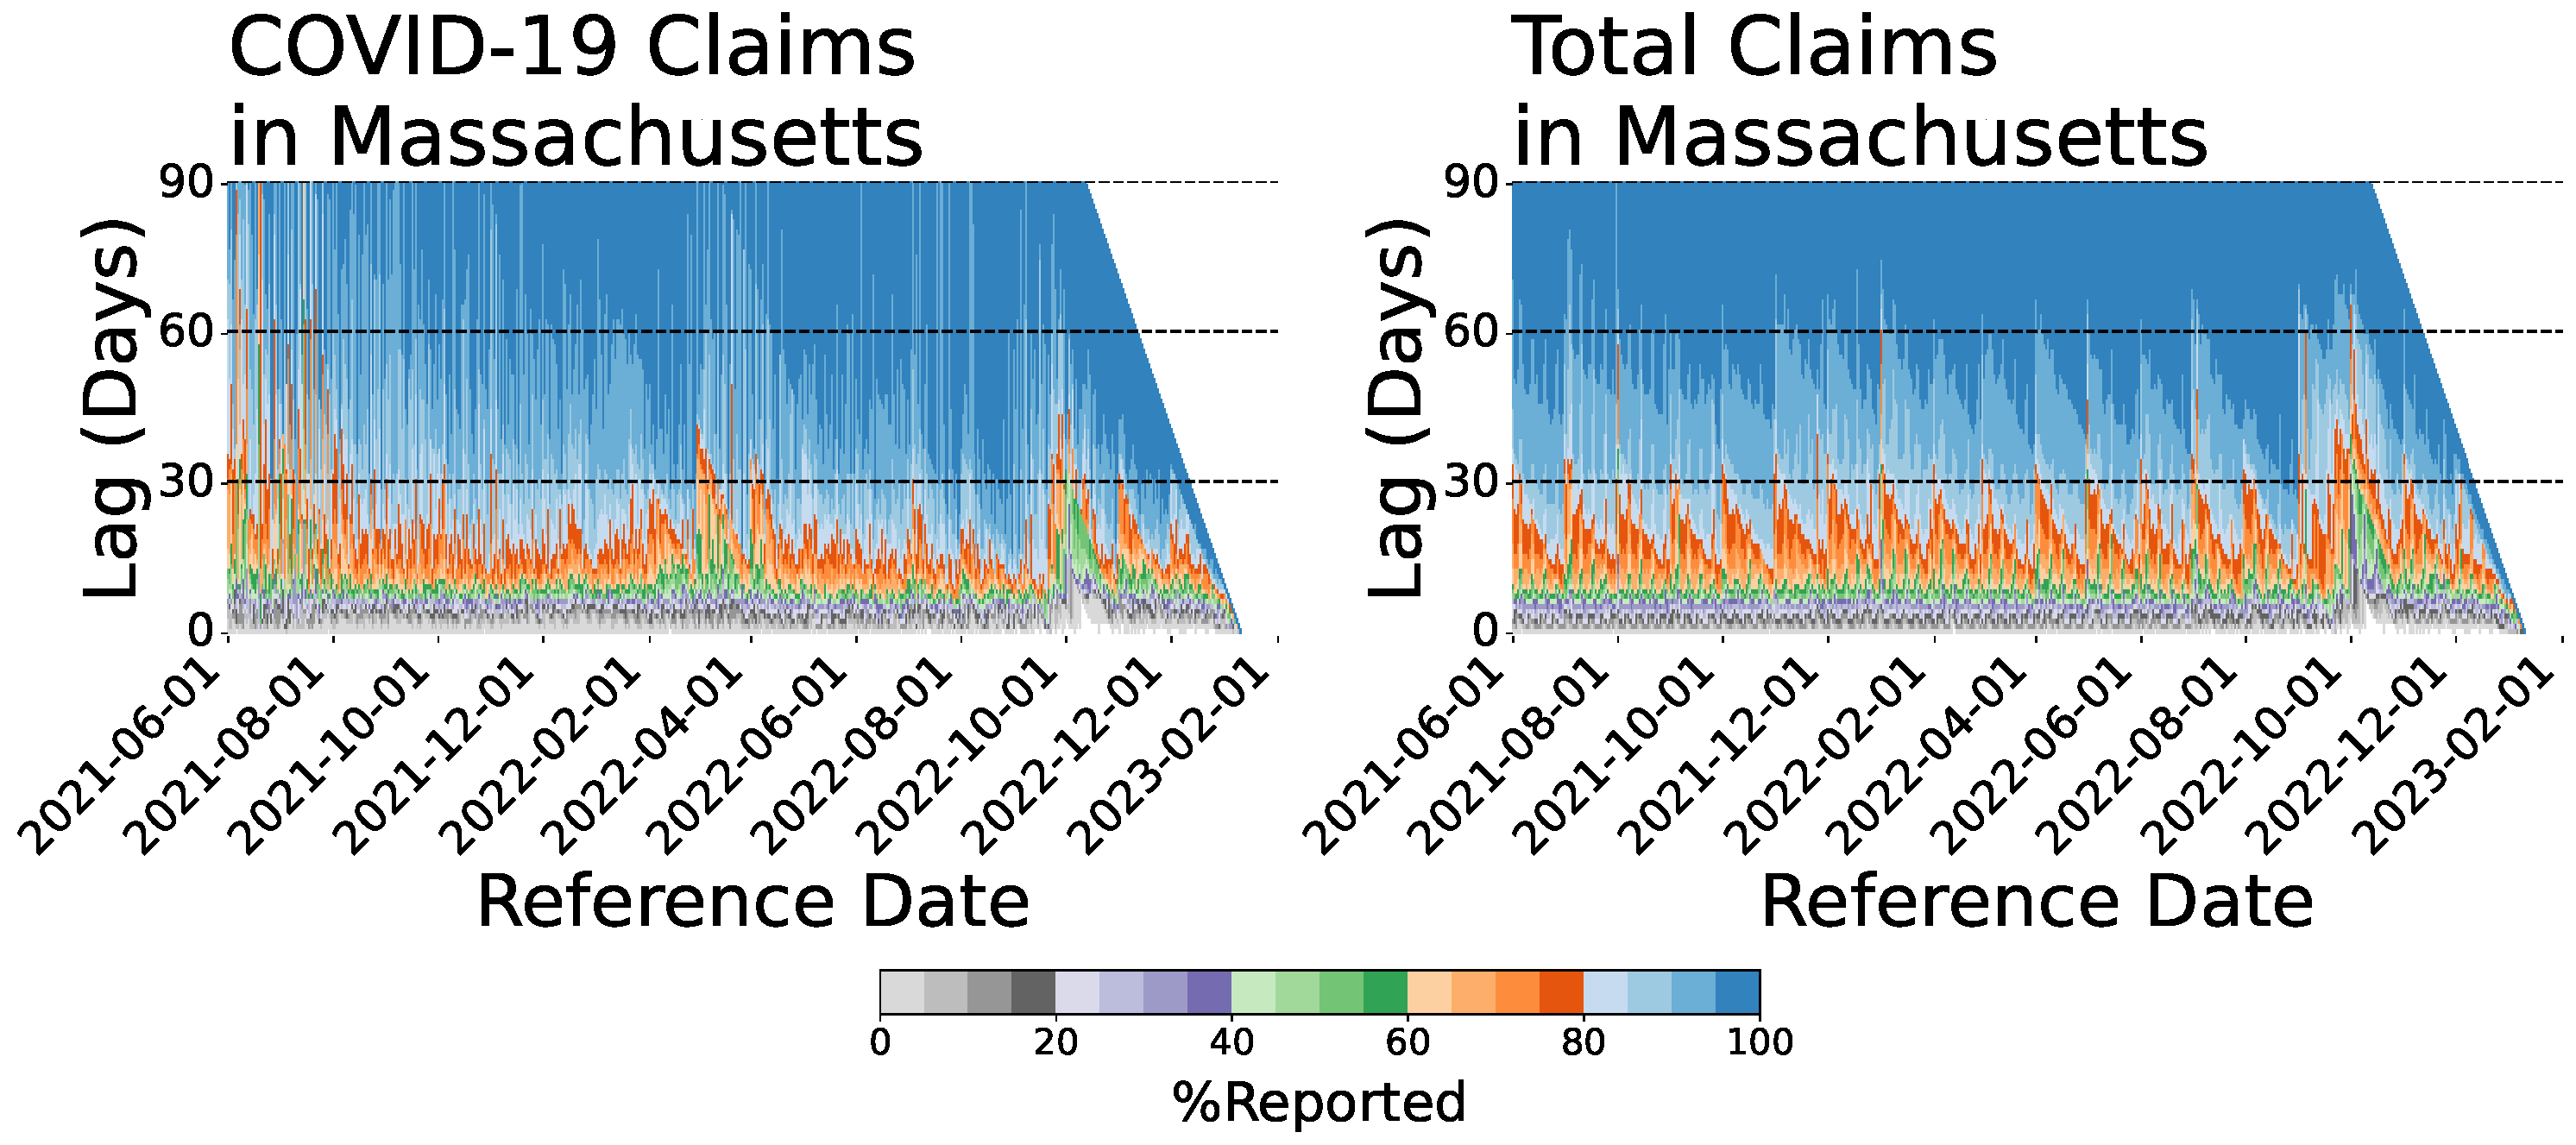
\includegraphics[width=\textwidth]{figs/completeness_Massachusetts.pdf}
    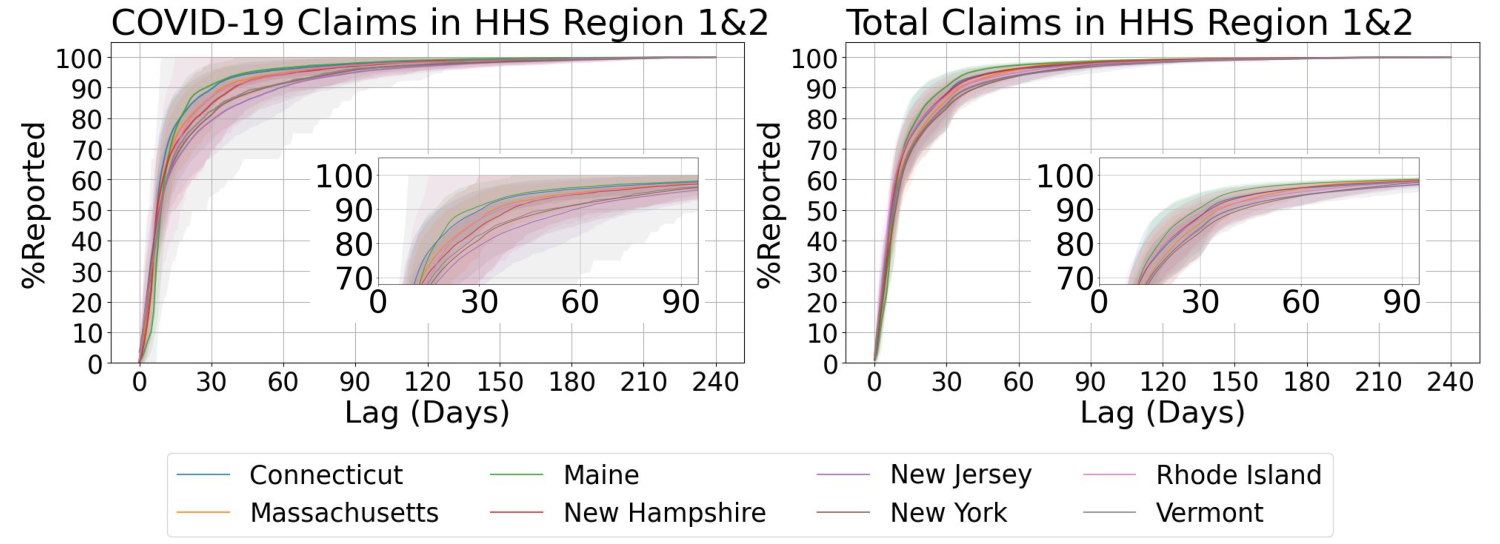
\includegraphics[width=\textwidth]{figs/completeness_lineplot_hhs1&2.pdf}
    \caption{\emph{Top: Distribution of the percentage of reported in Massachusetts, grouped by lag and recorded across reference dates. Bottom: Mean percentage of reported, averaged over all reference dates between 2021-06-01 and 2023-01-10, plotted by lag for states in HHS Regions 1 and 2. Shaded bands represent the 10th to 90th percentile interval. The left panel is based on CHNG outpatient COVID-19 claims data, while the right panel is based on CHNG outpatient total claims data.}}
\end{figure}

\paragraph{Selection of Target Lag $L$:}
To better understand the data revision patterns, we analyze the distribution of the variable \( p_{itl} \), defined as \( p_{itl} = Y_{itl} / Y_{itL_{it}} \), across reporting lags. For count-tyoe data (e.g., the number of confirmed cases), \( p_{itl} \times 100 \% \) quantifies the percentage of the total value reported at the \((l+1)\)th release for location \( i \) and reference date \( t \). For fraction-type data (e.g., the fraction of COVID-19 insurance claims), \( p_{itl} \) represents the normalized provisional estimate. Since the finalized value \( Y_{itL_{it}} \) is not observable in real time, we temporarily approximate it using a sufficiently large lag of 300, under the assumption that the revision process has effectively converged by that point. Specifically, we set $L_{it} = 300, Y_{itL_{it}} = Y_{it,300}$ to serve as a practical surrogate for the finalized target value.


The distribution of $p_{itl}$ provides insight into how data revision sequences evolve over time. In addition to the apparent day-of-week effect and week-of-month effect, the efficiency of data revision is significantly influenced during periods when the epidemic curve is at or near its peak. Figure 2 illustrates this phenomenon using CHNG outpatient insurance claim data in MA as an example. Overall, the revision of COVID-19 claims exhibit greater variance than non-COVID claims, underscoring the difficulty of the forecast task.

Although there may be a considerable degree of heterogeneity in $L_{it}$ (the target horizon for $Y_{it}$, example shown in Figure S1 in Appendix A), the most substantial revisions are typically made within the first two months for the majority locations including states and populous counties for CHNG outpatient insurance claims data. The bottom panel of Figure 2 shows an example based on CHNG outpatient COVID-19 insurance claims data. It reveals that, for states in HHS Region 1 and Region 2, almost all mean \%reported values for COVID-19 reach 90\% when the lag equals 60 days.  

In our experiments, we set \( L = 60 \) for the CHNG outpatient COVID-19 insurance claims data and \( L = 45 \) for the Quidel COVID-19 antigen tests data, both applied uniformly across all states considered. For the data on confirmed cases from MA-DPH, we set \( L = 14 \), ensuring that at least 90\% cases are reported while keeping \( L \) relatively small.

\paragraph{Training Frequency:}
We generate state-level forecasts following the adaptive modeling protocol described in Section 3.2. To improve computational efficiency, model training is performed every 30 days, except for the MA-DPH confirmed case forecasts, where the shorter target lag of 14 days requires retraining every 7 days. While this adjustment reduces computational cost, it may degrade predictive performance in the presence of non-stationarity—particularly in scenarios involving abrupt and substantial changes in data revision patterns—as less frequent retraining limits the model's ability to adapt in a timely manner. On each retraining date \( s_{\text{train}} \), the model is updated with newly available training data and subsequently used to generate quantile forecasts for all epidemic quantities reported on dates \( s \in [s_{\text{train}}, s_{\text{train}}+30) \) (or \( s \in [s_{\text{train}}, s_{\text{train}}+7) \) for the MA-DPH case forecasts).




\paragraph{Location-Specific Model Training:}
Both the CHNG outpatient insurance claims data and Quidel antigen tests data are subject to geographic variation in market share, health-seeking behavior, and reporting practices. These differences render the data incomparable across locations and result in location-specific revision patterns. In this study, we do not attempt to address spatial heterogeneity; instead, we fit the model separately for each location.










\subsection{Accuracy of Revision Forecasts}
In the subsequent analysis, we evaluate forecasting performance using the Weighted Interval Score (WIS). To reiterate, the WIS measures the distance between the forecast distribution and the observed target value on the log scale. The quantity \( \exp(\text{WIS}) - 1 \) provides an interpretable approximation of the absolute relative error. The arithmetic mean of WIS captures relative error in log space, which is equivalent to the geometric mean in the original scale. 

The forecasting performance is evaluated relative to a baseline model, defined as a flat-line predictor whose forecasted median is the 7-day moving average of the most recent observations. Consequently, the WIS for the baseline reduces to the absolute error on the log scale between the most recent observation and the finalized.

We evaluate the forecasting performance of our framework across the three datasets described in Section 4.1. For the MA-DPH confirmed cases, which are usually normalized by a constant (the MA population), we generate forecasts only for the counts. For the insurance claims, we produce forecasts for both the counts and the fractions of COVID-19–related outpatient claims. For the antigen tests, we forecast the fraction of positive tests among all tests conducted.


The following is a summary of the experimental results:
\begin{itemize}
    \item Our data revision forecasting framework substantially reduces forecast error, particularly at shorter lags (e.g., within the first 0–5 days). However, the marginal improvement diminishes as the lag increases. These results suggest that modeling and forecasting data revisions is most beneficial in settings where timely estimates are needed in near real-time.
    \item Comparing across the three datasets, we find that the task is most difficult for the insurance claims data, followed by antigent tests, and finally MA-DPH confirmed cases. Intuitively, this ordering matches Figure 1, where the claims data exhibit the slowest convergence among the three.
    \item Abrupt distributional shifts remain a significant challenge. Our model relies on historical data revision patterns to forecast future updates, which implicitly assumes that these patterns are stationary over time. When the revision process undergoes a sudden and substantial change—particularly one that has not been observed in the training data—the model may struggle to adapt, resulting in degraded forecasting performance. 

\end{itemize}

Next, we demonstrate the forecasting performance of our model and how the performance varies along difference dimensions. 

\begin{figure}[h!]
    \centering
    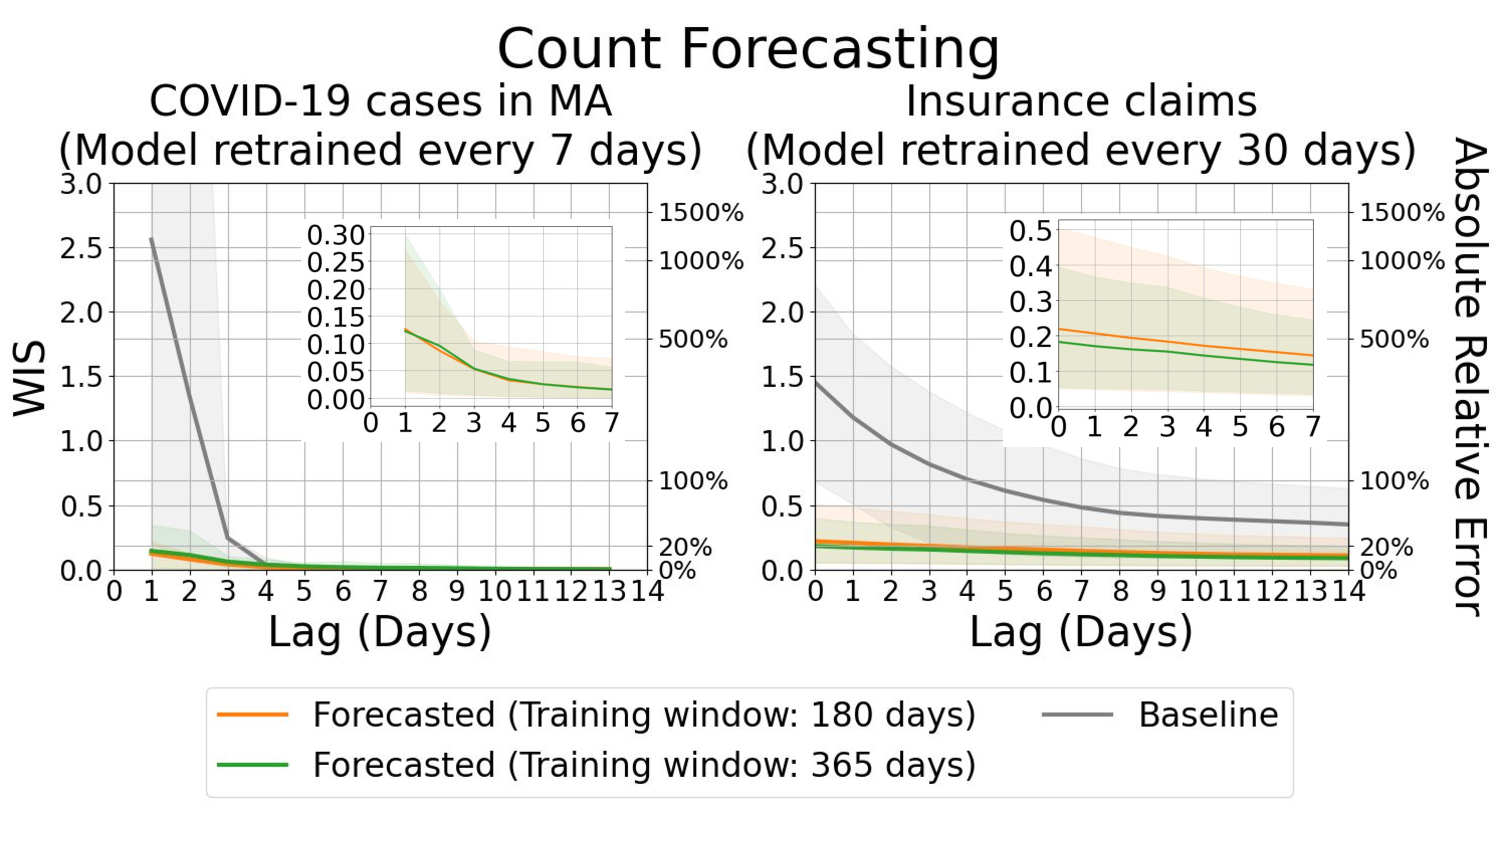
\includegraphics[width=\textwidth]{figs/experiment_count_result_evl_general.pdf}
    \caption{\emph{\textbf{Evaluation of forecasts for counts, aggregated by lag.} Left: Forecasts of finalized confirmed COVID-19 case counts in MA. Right: Forecasts of COVID-19 insurance claims across all states, based on CHNG outpatient insurance claims data. Solid lines indicate the mean WIS, which approximates absolute relative errors between the most recent report and the target, averaged over locations and reference dates for each lag. Shaded areas represent the 10th to 90th percentile interval.}}
\end{figure}

\begin{figure}[h!]
    \centering
    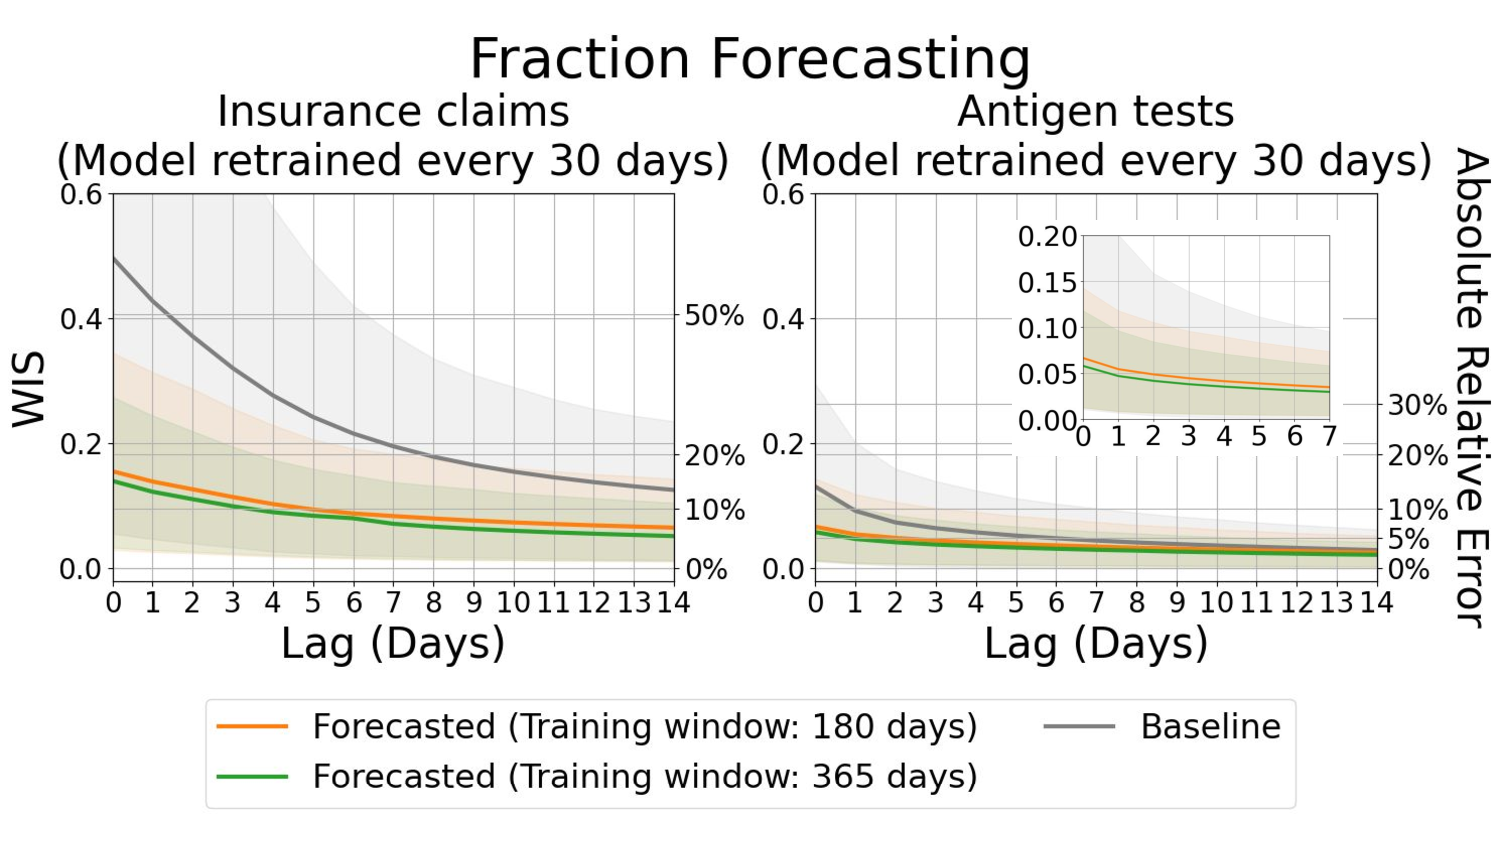
\includegraphics[width=\textwidth]{figs/experiment_fraction_result_evl_general.pdf}
    \caption{\emph{\textbf{Evaluation of forecasts for fractions, aggregated by lag.} Left: Forecasts of the fraction of COVID-19 insurance claims based on CHNG outpatient insurance claims data. Right: Forecasts of the fraction of positive COVID-19 antigen tests based on Quidel antigen tests data. Solid lines represent the mean WIS, , which approximates absolute relative errors between the most recent report and the target, averaged over locations and reference dates for each lag. Shaded areas indicate the 10th to 90th percentile interval.}}
\end{figure}

\subsection{Aggregate Accuracy by Lag}
We investigate how forecasting performance varies as a function of the lag at which the report (or the revision) is made. For a given report date \( s \), we define the forecasting task as having a lag of \( s - t \) when predicting \( Y_{itL} \) using all data available up to and including date \( s \). Since the revision sequence of \( Y_{it} \) gradually converges to its finalized value, forecasts made with shorter lags are inherently more challenging due to the limited availability of information in earlier stages.

Figure 3 and Figure 4 present the evaluation results for count and fraction forecasts, respectively, stratified by lag and averaged over all locations and reference dates. For confirmed cases from MA-DPH (Figure3, left panel), the mean WIS of the baseline model begins at approximately 2.56 when the lag is 1, corresponding to a mean absolute relative error of roughly 1189.43\% under this evaluation metric. In contrast, the mean WIS of our distributional forecasts is substantially lower—0.12 (approximately 13.04\% absolute relative error) when using a 180-day training window, and 0.14 (approximately 15.55\%) when using a 365-day training window. These results demonstrate that our approach outperforms the baseline, particularly when the lag is less than 4 days.

The performance gap is even more pronounced for the insurance claims data, where revision patterns tend to be more frequent and variable. As shown in the right panel of Figure 3, the baseline model maintains a mean WIS above 0.18—corresponding to an absolute relative error of approximately 20\%—even after 14 days of revision. In comparison, our model yields a mean WIS of 0.23 (approximately 25.65\% absolute relative error) at lag 0 (i.e., the first data release) when using a 180-day training window, and 0.20 (approximately 22.65\%) with a 365-day training window. After 14 days of revision, the forecasting accuracy improves with our model achieving a mean WIS of 0.12 (approximately 12.70\% absolute relative error) using the 180-day window, and 0.10 (approximately 10.80\% absolute relative error) using the 365-day window.

Similarly, Figure 4 illustrates the evaluation results of COVID-19 fraction forecasts as a function of lag. For insurance claims data, the mean WIS exceeds 0.45 which approximates an absolute relative error of around 56.83\% when comparing the first release (lag = 0) to the target (lag = 60). However, this mean WIS is reduced to around 0.16  (approximately 16.79\% absolute relative error) using our distributional forecasts with a 180-day training window and a mena WIS of 0.14 (approximately 15.00\% absolute relative error) with a 365-day training window. Even after 7 days of revisions, the distributional forsecasts continue to yield substantial improvements. 

In contrast, the antigen tests are considerably less affected by the data revision problem. Nevertheless, even when provisional reports closely approximate the target, our framework still achieves substantial improvements in forecast accuracy. Specifically, at the first release (lag = 0), the mean WIS decreases from approximately 0.13 (corresponding to a 13.95\% absolute relative error) to 0.07 (6.88\% absolute relative error) when using a 180-day training window, and further to 0.06 (5.97\% absolute relative error) when using a 365-day training window.

\subsection{Aggregate Accuracy by Reference Date}

\begin{figure}[h!]
    \centering
    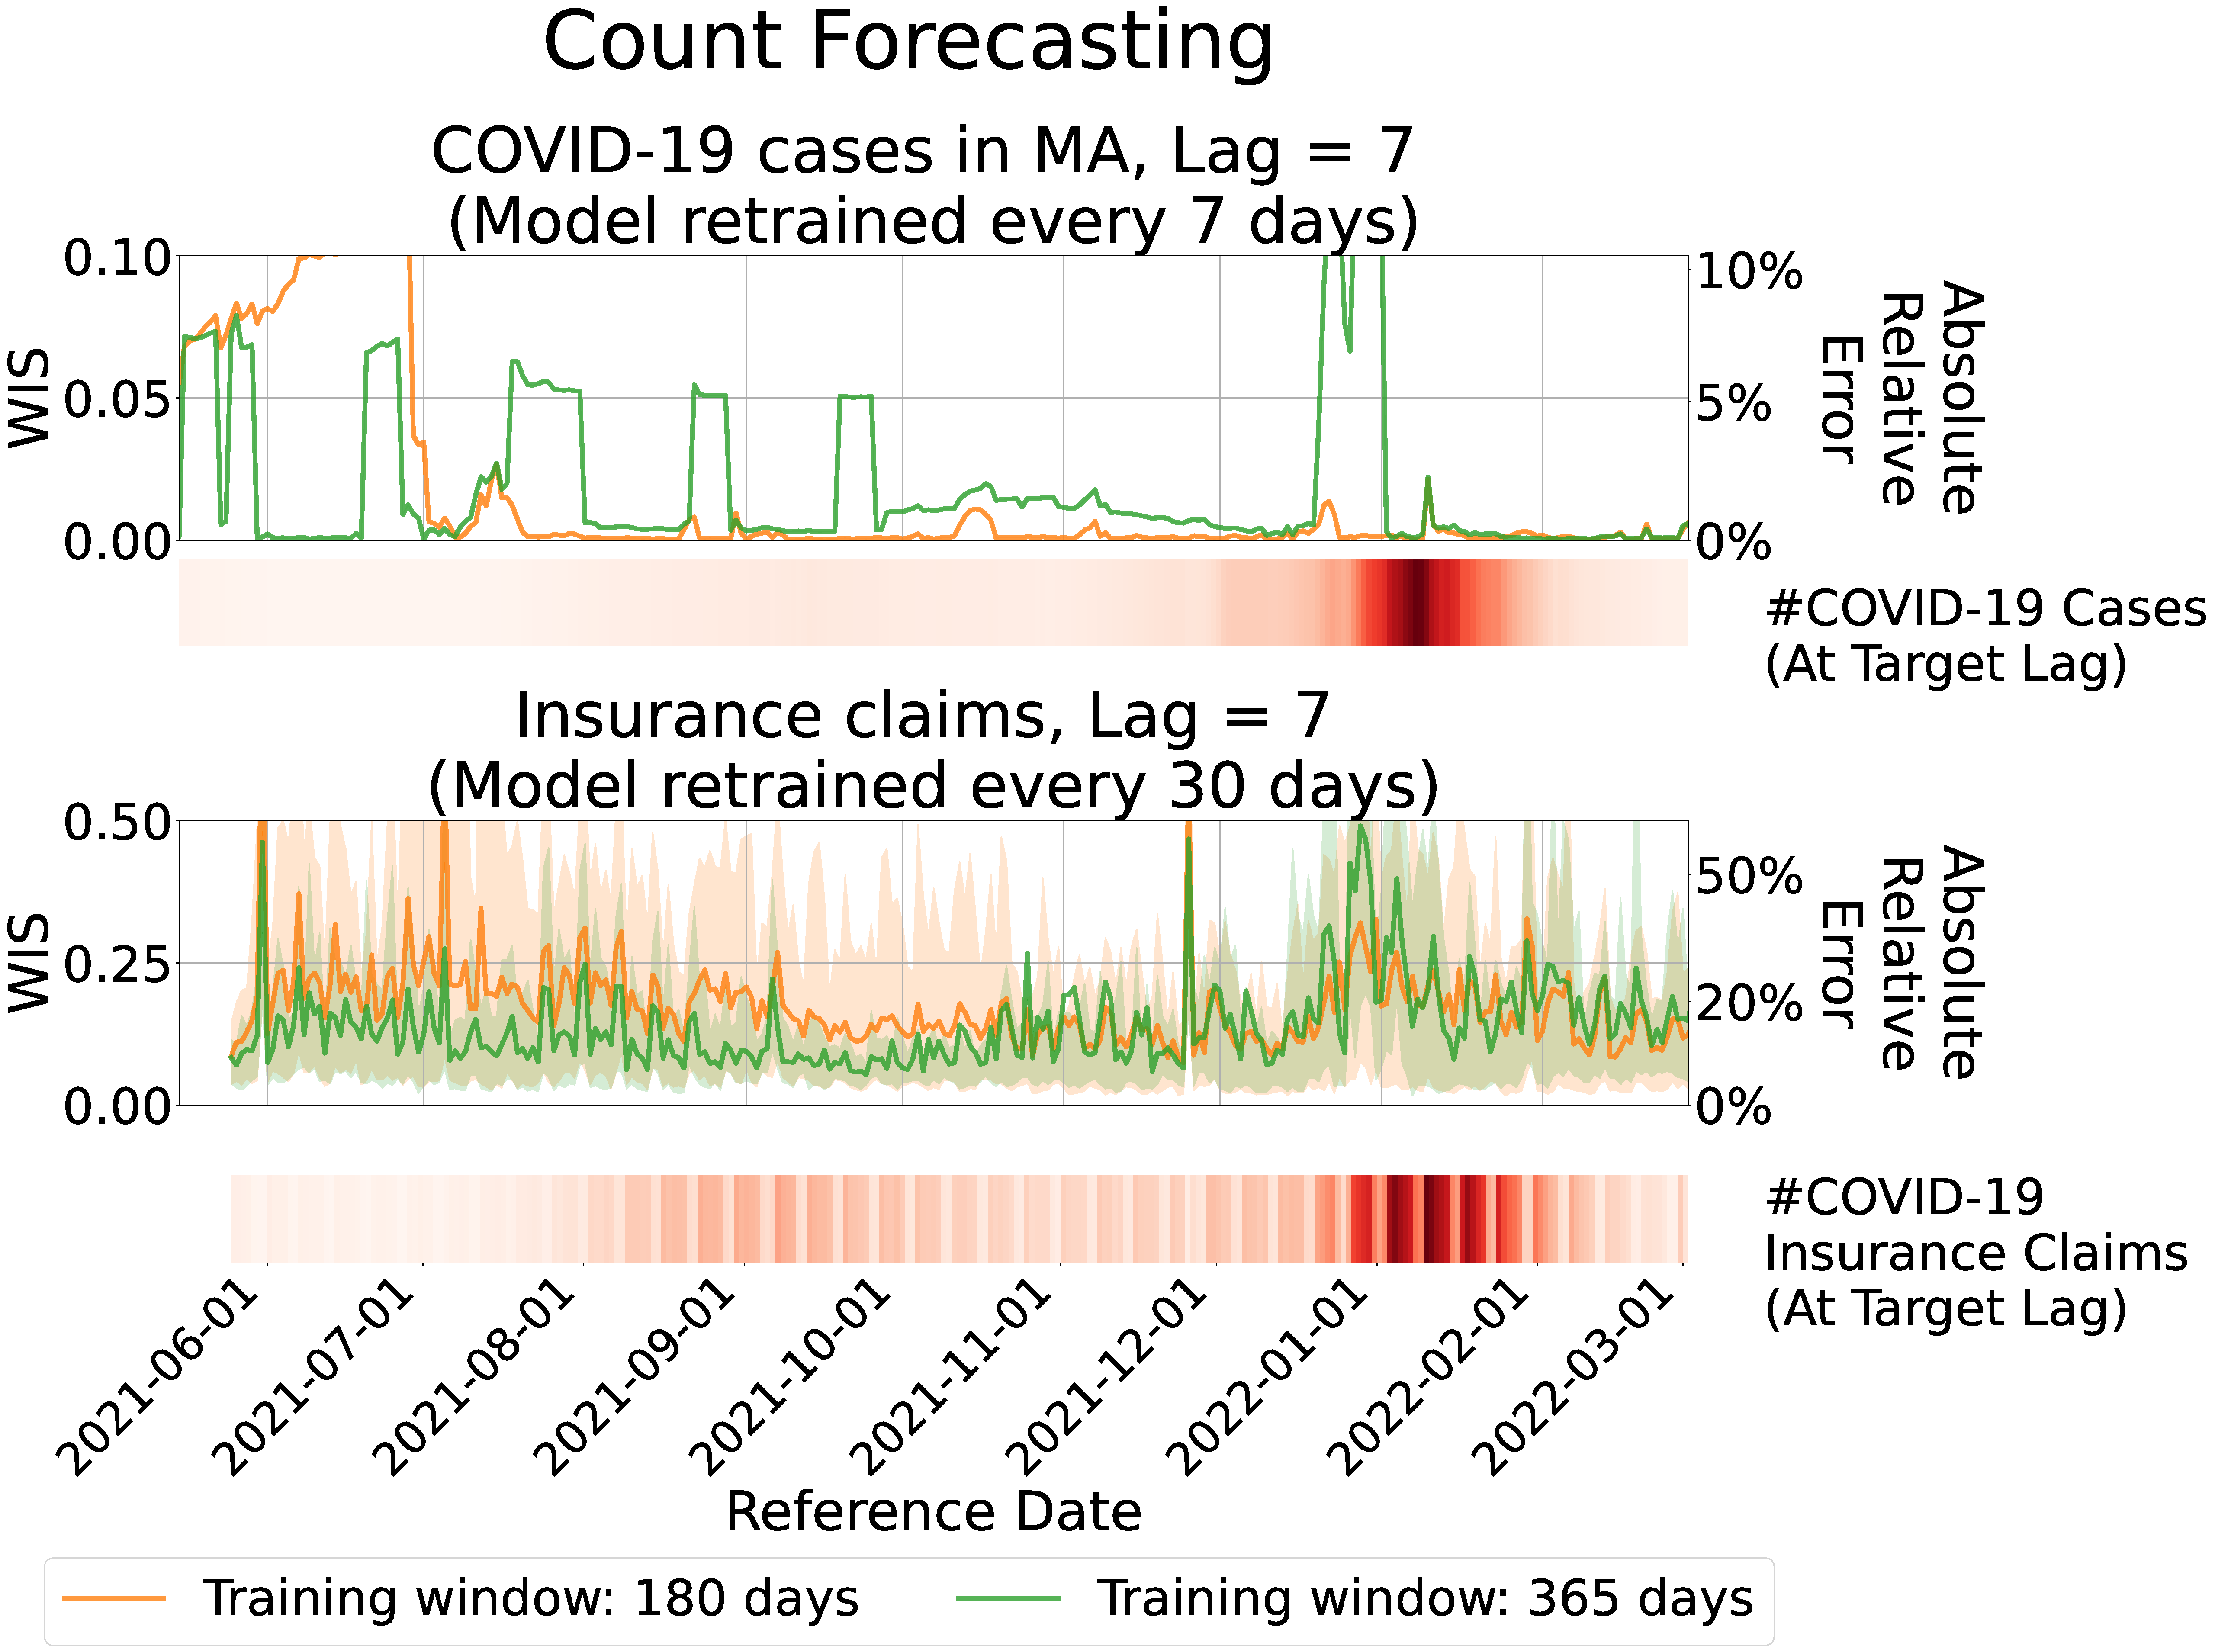
\includegraphics[width=\textwidth]{figs/experiment_count_result_time_series.pdf}
    \caption{\emph{\textbf{Evaluation of forecasts for counts, aggregated by reference date} Top: Forecasts of finalized confirmed COVID-19 case counts in MA. Bottom: Forecasts of COVID-19 insurance claims across all states, based on CHNG outpatient insurance claims data. Solid lines represent the mean WIS at lag 7, averaged over locations for each reference date. Shaded areas indicate the 10th to 90th percentile interval. The accompanying heatmaps display the corresponding target values, with darker shades indicating larger number of cases or claim counts.}}
\end{figure}

\begin{figure}[h!]
    \centering
    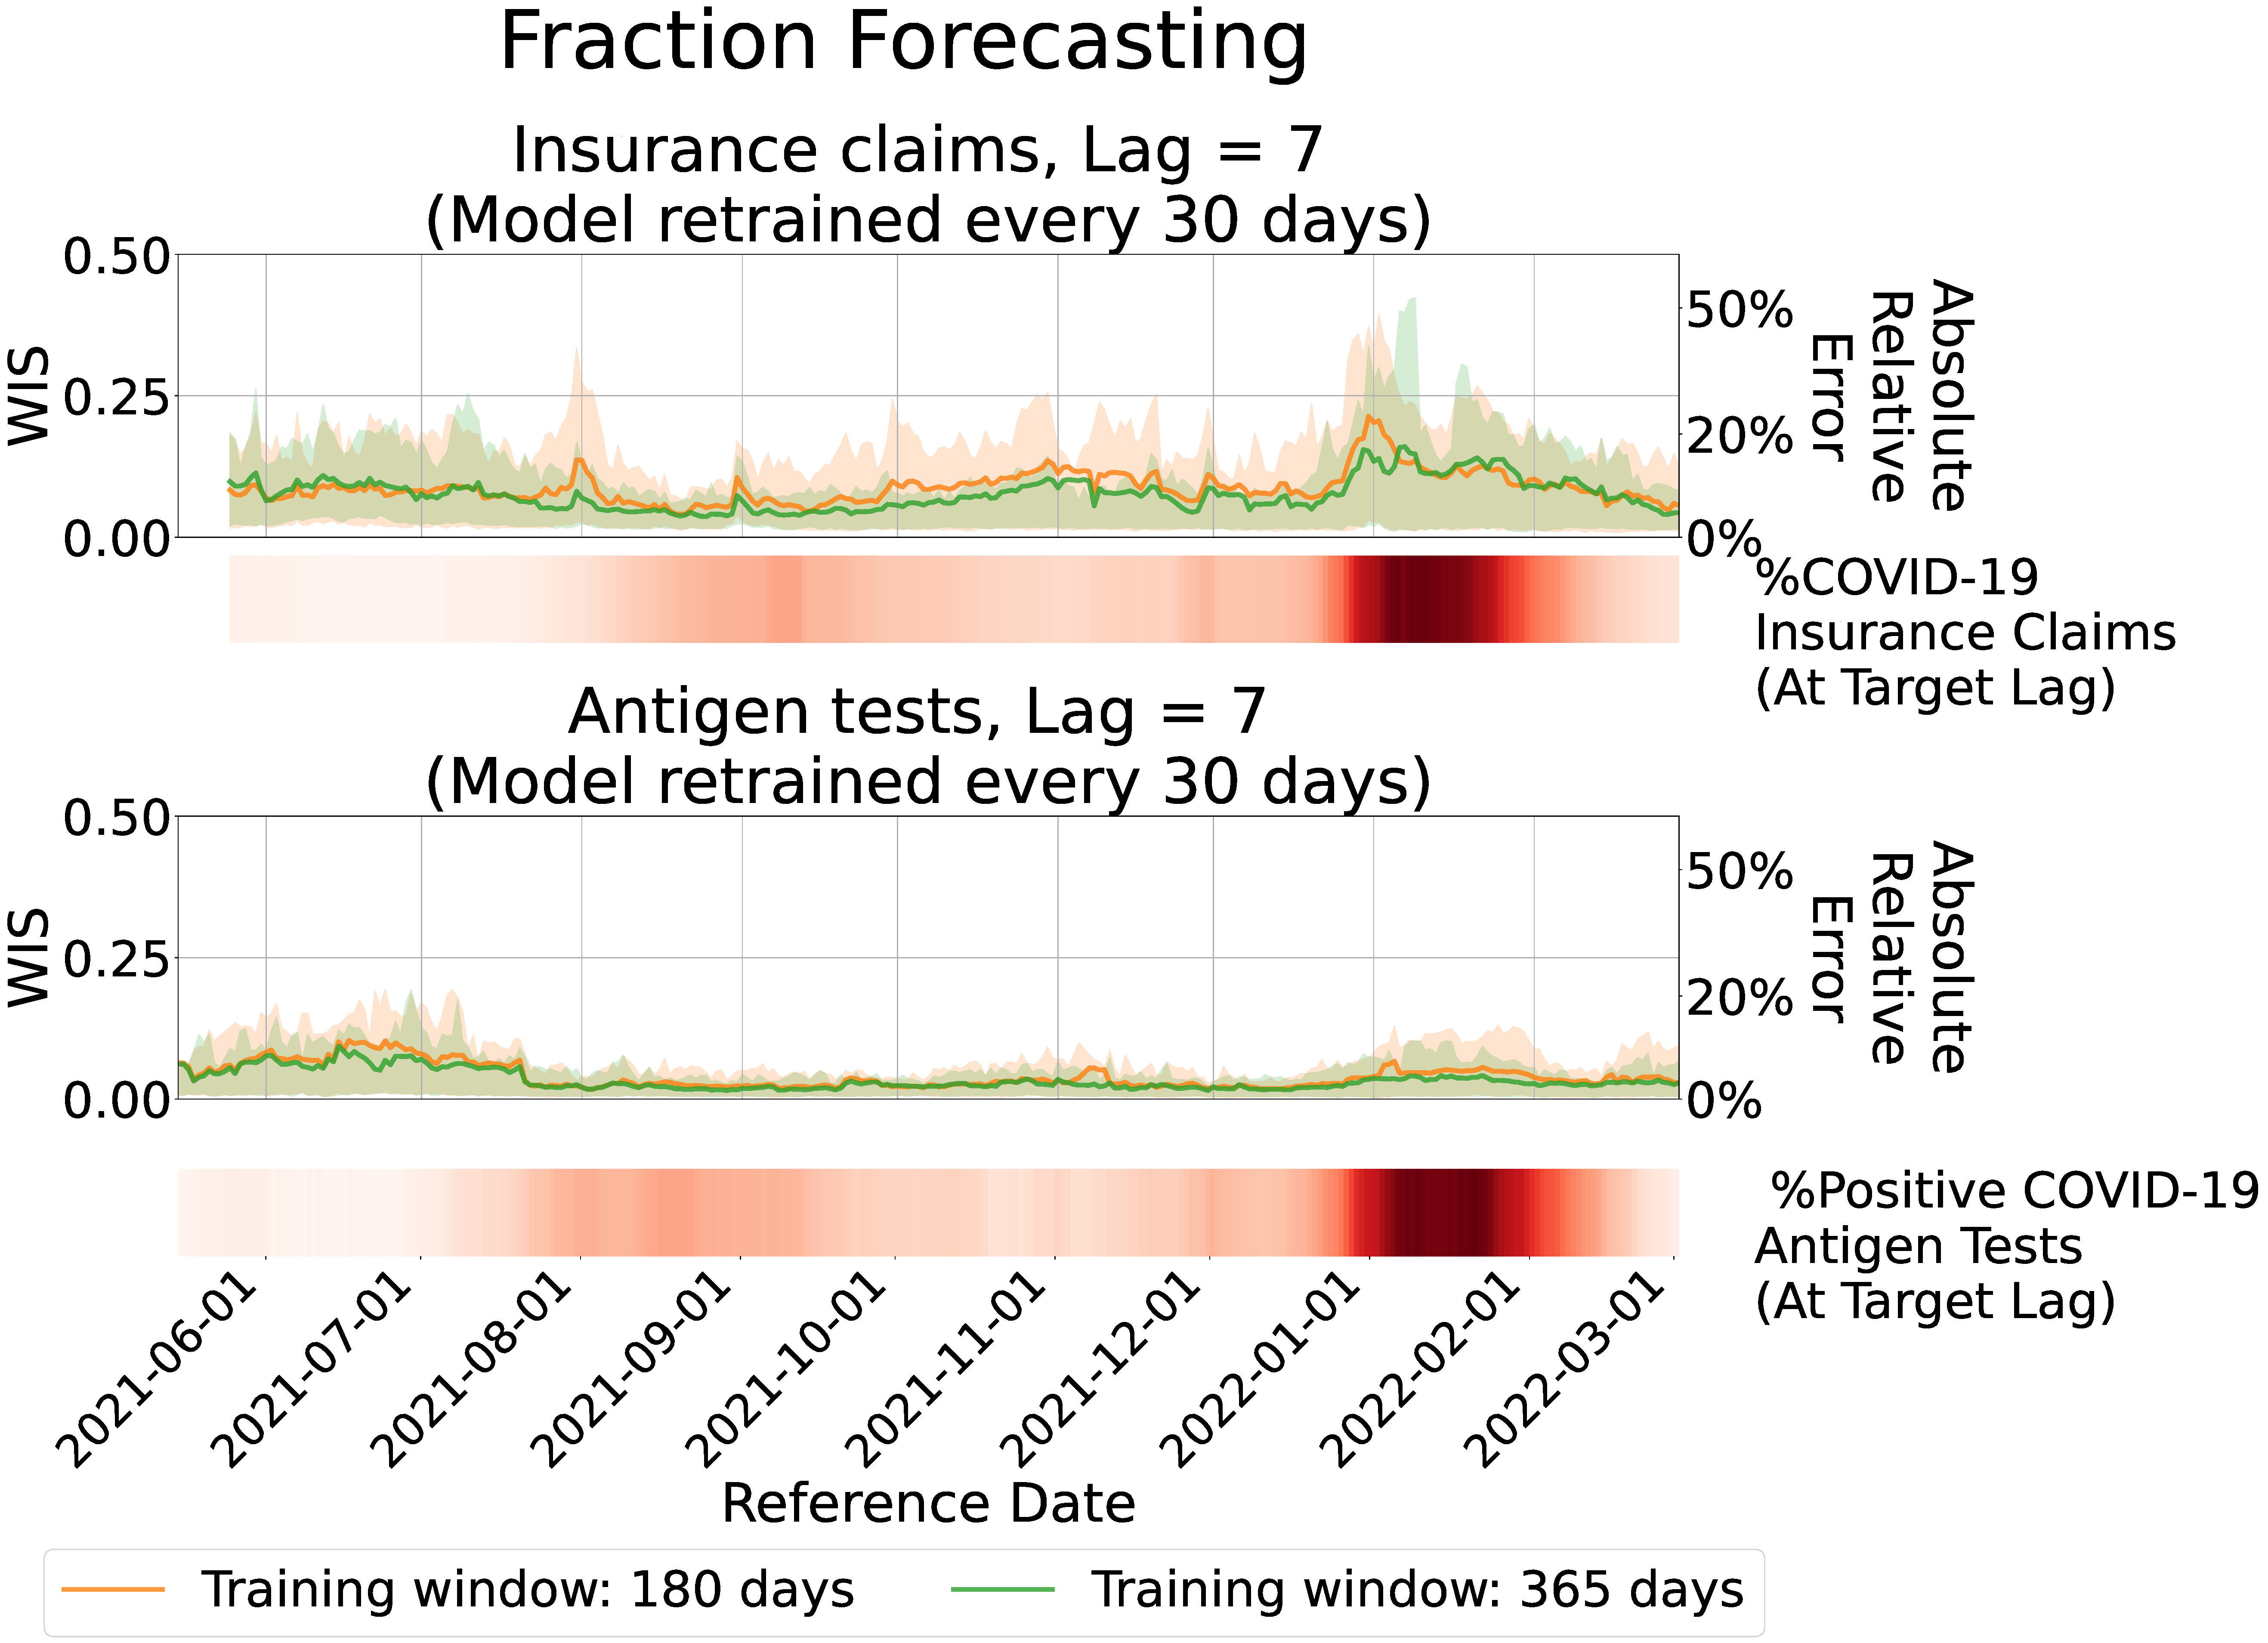
\includegraphics[width=\textwidth]{figs/experiment_fraction_result_time_series.pdf}
    \caption{\emph{\textbf{Evaluation of forecasts for fractions, aggregated by reference date.} Top: Forecasts of the fraction of COVID-19 insurance claims based on CHNG outpatient insurance claims data. Bottom: Forecasts of the fraction of positive COVID-19 antigen tests based on Quidel antigen tests data. Solid lines represent the mean WIS at lag 7, averaged over locations for each reference date. Shaded areas indicate the 10th to 90th percentile interval. The accompanying heatmaps display the target values, with darker shades indicating higher fractions.}}
\end{figure}

The difficulty of the forecasting task varies not only with lag but also over time. Figure 5 and Figure 6 present evaluation results for forecasts made for reference dates from 2021-06-01 to 2022-03-01 at a fixed lag of 7 days, corresponding to count and fraction targets, respectively. The results are stratified by reference date and averaged across all locations. In each figure, the color strip (i.e., a one-dimensional heatmap below the line plot) indicates the target values over time.

Our model generally performs well. A comprehensive set of time series forecast evaluation results for all 50 states is provided in Appendix C. However, the forecast accuracy occasionally declines during periods of rapid epidemiological change, particularly during the Omicron wave (November 2021 to February 2022). This degradation is primarily due to the lagged nature of the model: coefficients estimated from data observed \( L \) days earlier may not adequately capture abrupt shifts in revision patterns, resulting in reduced performance under non-stationary conditions.

The Omicron wave, the largest observed during the COVID-19 pandemic, was characterized by unprecedented infection rates and severe strain on public health reporting systems. In contrast to the preceding Delta wave (July to November 2021), the Omicron surge induced abrupt and substantial changes in the data revision pattern. These shifts posed a significant challenge for our model, which struggled to adapt to revision dynamics not previously encountered in the training data.

Another challenging period is from June to July 2021, characterized by an extremely low general infection rate. Recall that the WIS consists of absolute deviations between the forecasts and the target. This evaluation metric will exaggerate relative errors when the target is extremely small.


\subsection{Impact Factors of Forecast Accuracy}
Our method exhibits degraded performance under two specific scenarios: (1) periods marked by abrupt changes in the target surveillance trend, and (2) periods when the target values are extremely small. The first scenario relates to the direction of the trend in the target surveillance curve, while the second pertains to the magnitude of the target values. We now examine the distribution of WIS across different lags, conditioned separately on each of these two factors, using the CHNG outpatient COVID-19 fraction data as a case study.

The left panel of Figure 7 shows the distribution of WIS across different lags, stratified by the trend direction of the CHNG outpatient COVID-19 fraction. We classify each instance into one of three categories: increasing (“up”), decreasing (“down”), or stable (“flat”) trends. The trend indicator \( Z_{it} \) is defined as:

\[
Z_{it} =
\begin{cases}
    1, & \text{if } \frac{\widetilde{Y}_{itL}}{\widetilde{Y}_{i(t-7)L}} \geq 1.25 \\
    -1, & \text{if } \frac{\widetilde{Y}_{itL}}{\widetilde{Y}_{i(t-7)L}} \leq 0.75 \\
    0, & \text{otherwise}
\end{cases}
\]

We assign \( Z_{it} = 1 \) if the 7-day average of the target value has increased by at least 25\% relative to the previous week, indicating an upward trend for location \( i \) at date \( t \). Conversely, \( Z_{it} = -1 \) denotes a decrease of at least 25\%, indicating a downward trend. All other cases are classified as flat (\( Z_{it} = 0 \)).



\begin{figure}[h!]
    \centering
    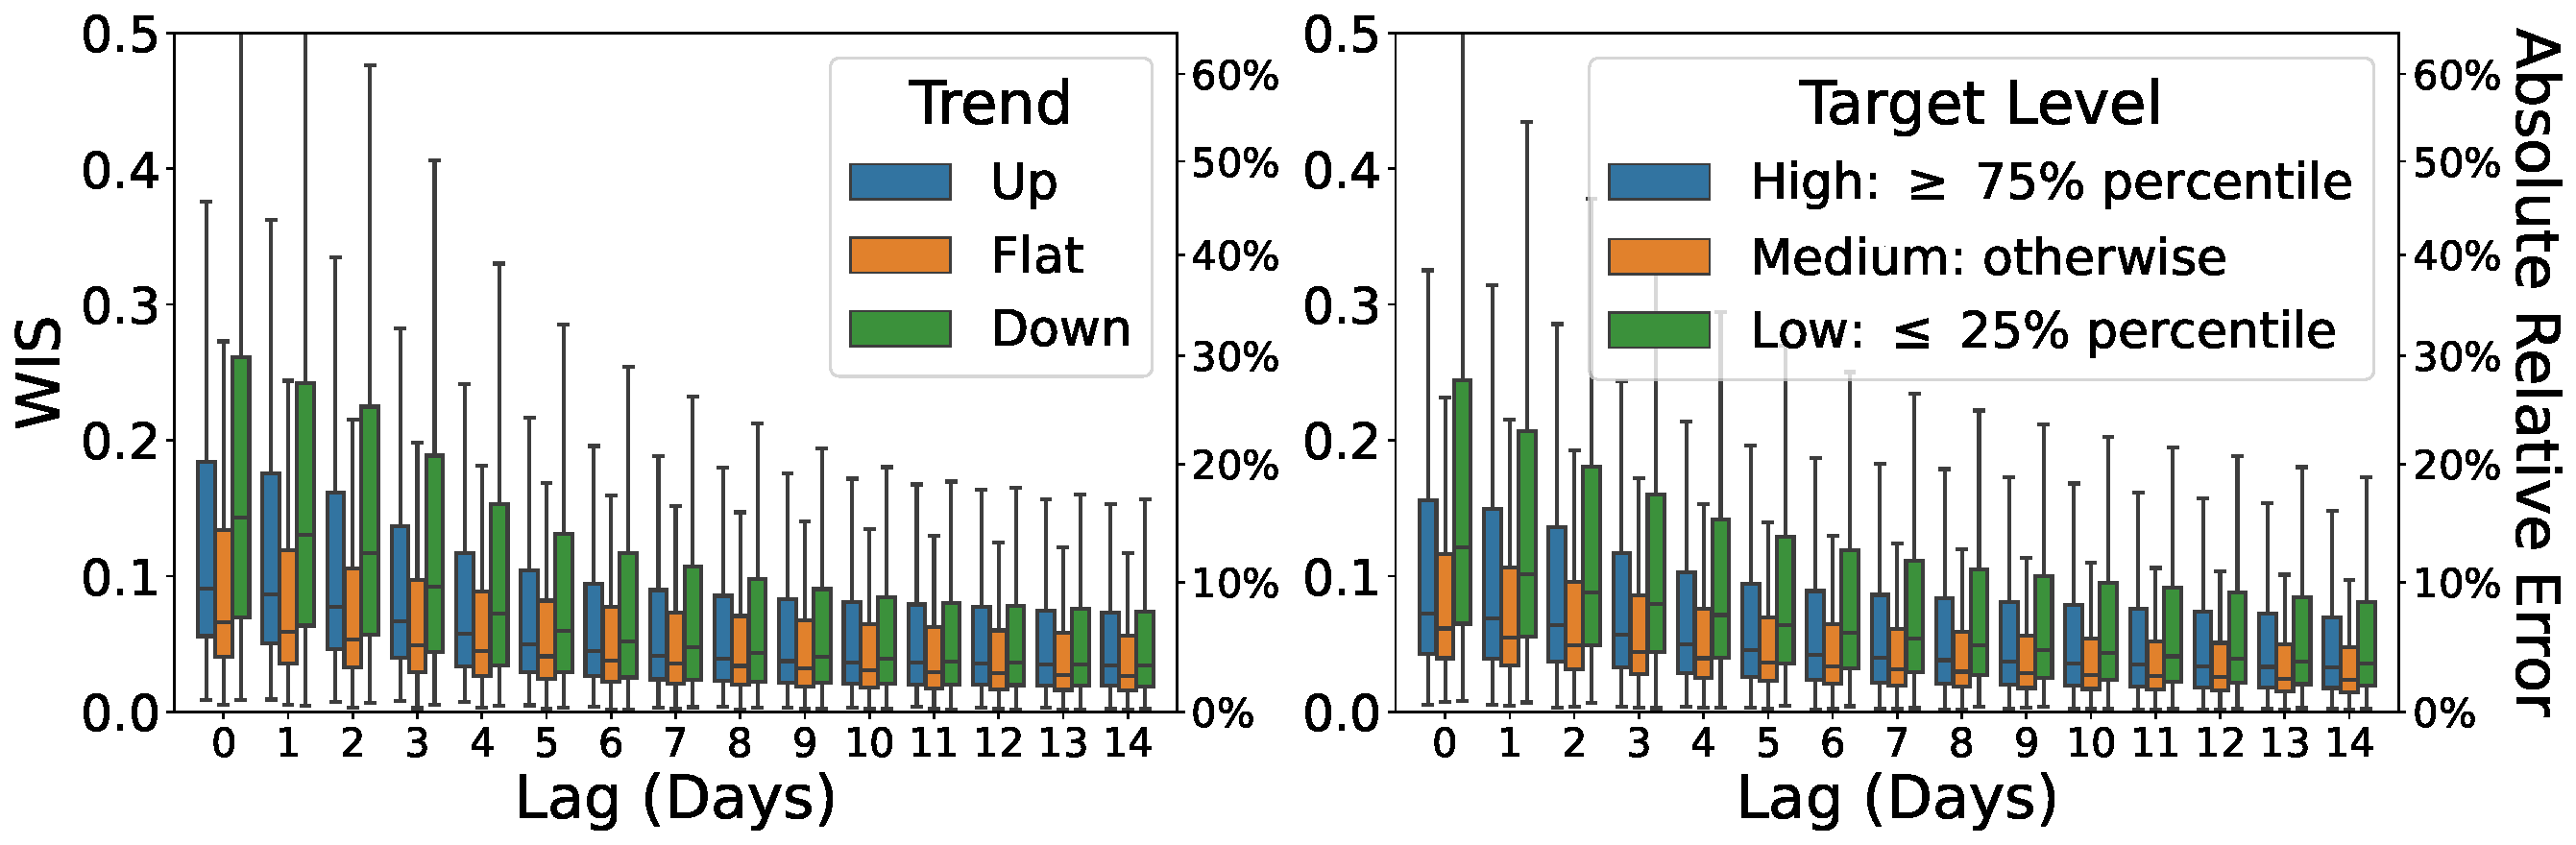
\includegraphics[width=\textwidth]{figs/experiment_fraction_result_factors.pdf}
    \caption{\emph{\textbf{Boxenplots illustrating the impact of surveillance conditions on forecast accuracy} (Each box displays the 25th, 50th (median), and 75th percentiles of the WIS). Left: Forecasts stratified by the direction of the target surveillance trend—"Up", "Flat", or "Down". Right: Forecasts stratified by the magnitude of the target, categorized as "High", "Medium", or "Low".}}
\end{figure}

Forecasting performance notably improves during periods with minimal changes in the target surveillance curve. The performance is the poorest during “Down” periods for quantities with only 0–7 revisions. This can be attributed to the fact that the “Down” category primarily corresponds to the downswing of the Omicron wave, whereas the “Up” category includes reference dates from the upswings of both the Delta and Omicron waves (as shown in Figure S52 in Appendix D). Overall, the model performs better during the Delta wave than during the Omicron wave, as the magnitude of distributional shift in the data revision pattern during Delta was comparatively smaller. After the first 7 revisions, the performance gap across the three trend categories narrows, with the performance ranking shifting to: “Flat”, “Down” and then “Up”.

The right panel of Figure 7 illustrates the distribution of WIS over lags, stratified by whether the target surveillance value falls into the categories of "High", "Medium", or "Low". A target value is classified as "High" if it is greater than or equal to the 75\% percentile, while it is classified as "Low" if it is less than or equal to the 25\% percentile. The performance order, from best to worst, consistently ranks as "Medium", "High", "Low" across lags. Notably, even after the first 14 revisions, the performance gap across these three categories remains significant.


\subsection{Comparison of Performance with Alternative Methods}
In this section, we demonstrate that our model achieves forecast accuracy comparable to, or exceeding, that of NobBS\cite{McGough2020} and Epinowcast\cite{epinowcast}, while substantially reducing computational runtime. These two methods were selected for comparison as they are among the most established in the literature, widely used in public health research projects, and supported by well-maintained R packages.

Since both methods are specifically designed for count-type data, our comparison is limited to count-type datasets. For the COVID-19 insurance claims with daily observations, we use a 180-day training window and a target lag of 60 days. To ensure a fair comparison, we apply the same 180-day moving window and a maximum delay of 60 days to NobBS and Epinowcast. To manage computational demands while maintaining consistency across models, we train all methods—including Delphi-RF—at 30-day intervals. Additionally, we evaluate performance on daily confirmed cases from MA-DPH, where revisions stabilize more quickly. For this dataset, we adjust the training frequency to every 7 days, set the maximum delay to 14 days, and maintain the 180-day moving window. In Delphi-RF, the target lag is also set to 14 days to align with these adjustments.

We further extend our comparison to weekly data. To ensure compatibility with weekly data, covariates containing daily change information were excluded. The full model is expressed as:

\begin{align*} 
&Q_{f(Y_{itL}))|X_{itl}}^{\tau} \\
=  &X_{itl}\beta^{\tau}\\
 = &\beta_0^{\tau}  + \mathbf{I}_{\text{first-week}(t+l)}\beta_{1}^{\tau} &&(\text{Intercept, week-of-month effects})\\ 
& + f(Y_{itl})\beta_{2}^{\tau} + \mathbf{e}_{\sqrt{Y_{itl}}}\beta_{3:5}^{\tau} &&(\text{Disease activity level}) \\ 
&+ \left(f(Y_{i(t-7)(l+7)}) - f(Y_{i(t-7)l_{\text{min}}})\right) \beta_{6}^{\tau}
&& \text{(Recent revision magnitude, \(t{-}7\))} \\
&+ \left(f(Y_{i(t-14)(l+14)}) - f(Y_{i(t-14)l_{\text{min}}})\right) \beta_{7}^{\tau}
&& \text{(Recent revision magnitude, \(t{-}14\))} \\
& + f(Y_{i(t-7)(l+7)}) \beta_{8}^{\tau} + f(Y_{i(t-14)(l+14)}) \beta_{9}^{\tau}
&& \text{(Short-term epidemic trends)}\\
\end{align*}

where \(Y_{itl}\) represents the counts reported for the week spanning reference dates \(t-6\) to \(t\), as of the report date \(t+l\), for location \(i\). 

To further evaluate model performance across diverse surveillance settings, we test the models on two additional datasets with distinct characteristics to assess their robustness. First, we apply the models to Puerto Rico (PR) dengue weekly surveillance data spanning from 1991-12-23 to 2010-11-29 (989 weeks). This dataset features a long historical record and strong seasonality, differs from the more irregular trends observed in COVID-19 data. Applying our method to the dengue data enables assessment of its ability to capture seasonal dynamics and long-term surveillance patterns. The target lag is set to 10 weeks, with 104 weeks of data used for training. For comparison, weekly forecasts are generated using NobBS and Epinowcast over the same time period. The maximum reporting delay is set to 10 weeks, and a 104-week moving window is applied, consistent with the setup in\cite{McGough2020}. For all three models, training and forecasting were conducted on a weekly basis.

We also test the models on national weekly influenza-like illness (ILI) case counts from 2014-06-30 to 2017-09-25 (170 weeks), which follow a distinct reporting pattern. For Delphi-RF, a 27-week training window is used with a target lag of 26 weeks. NobBS and Epinowcast are similarly configured with a 26-week maximum delay and a 27-week moving window, following the same settings in\cite{McGough2020}.


\begin{figure}[h!]
    \centering
    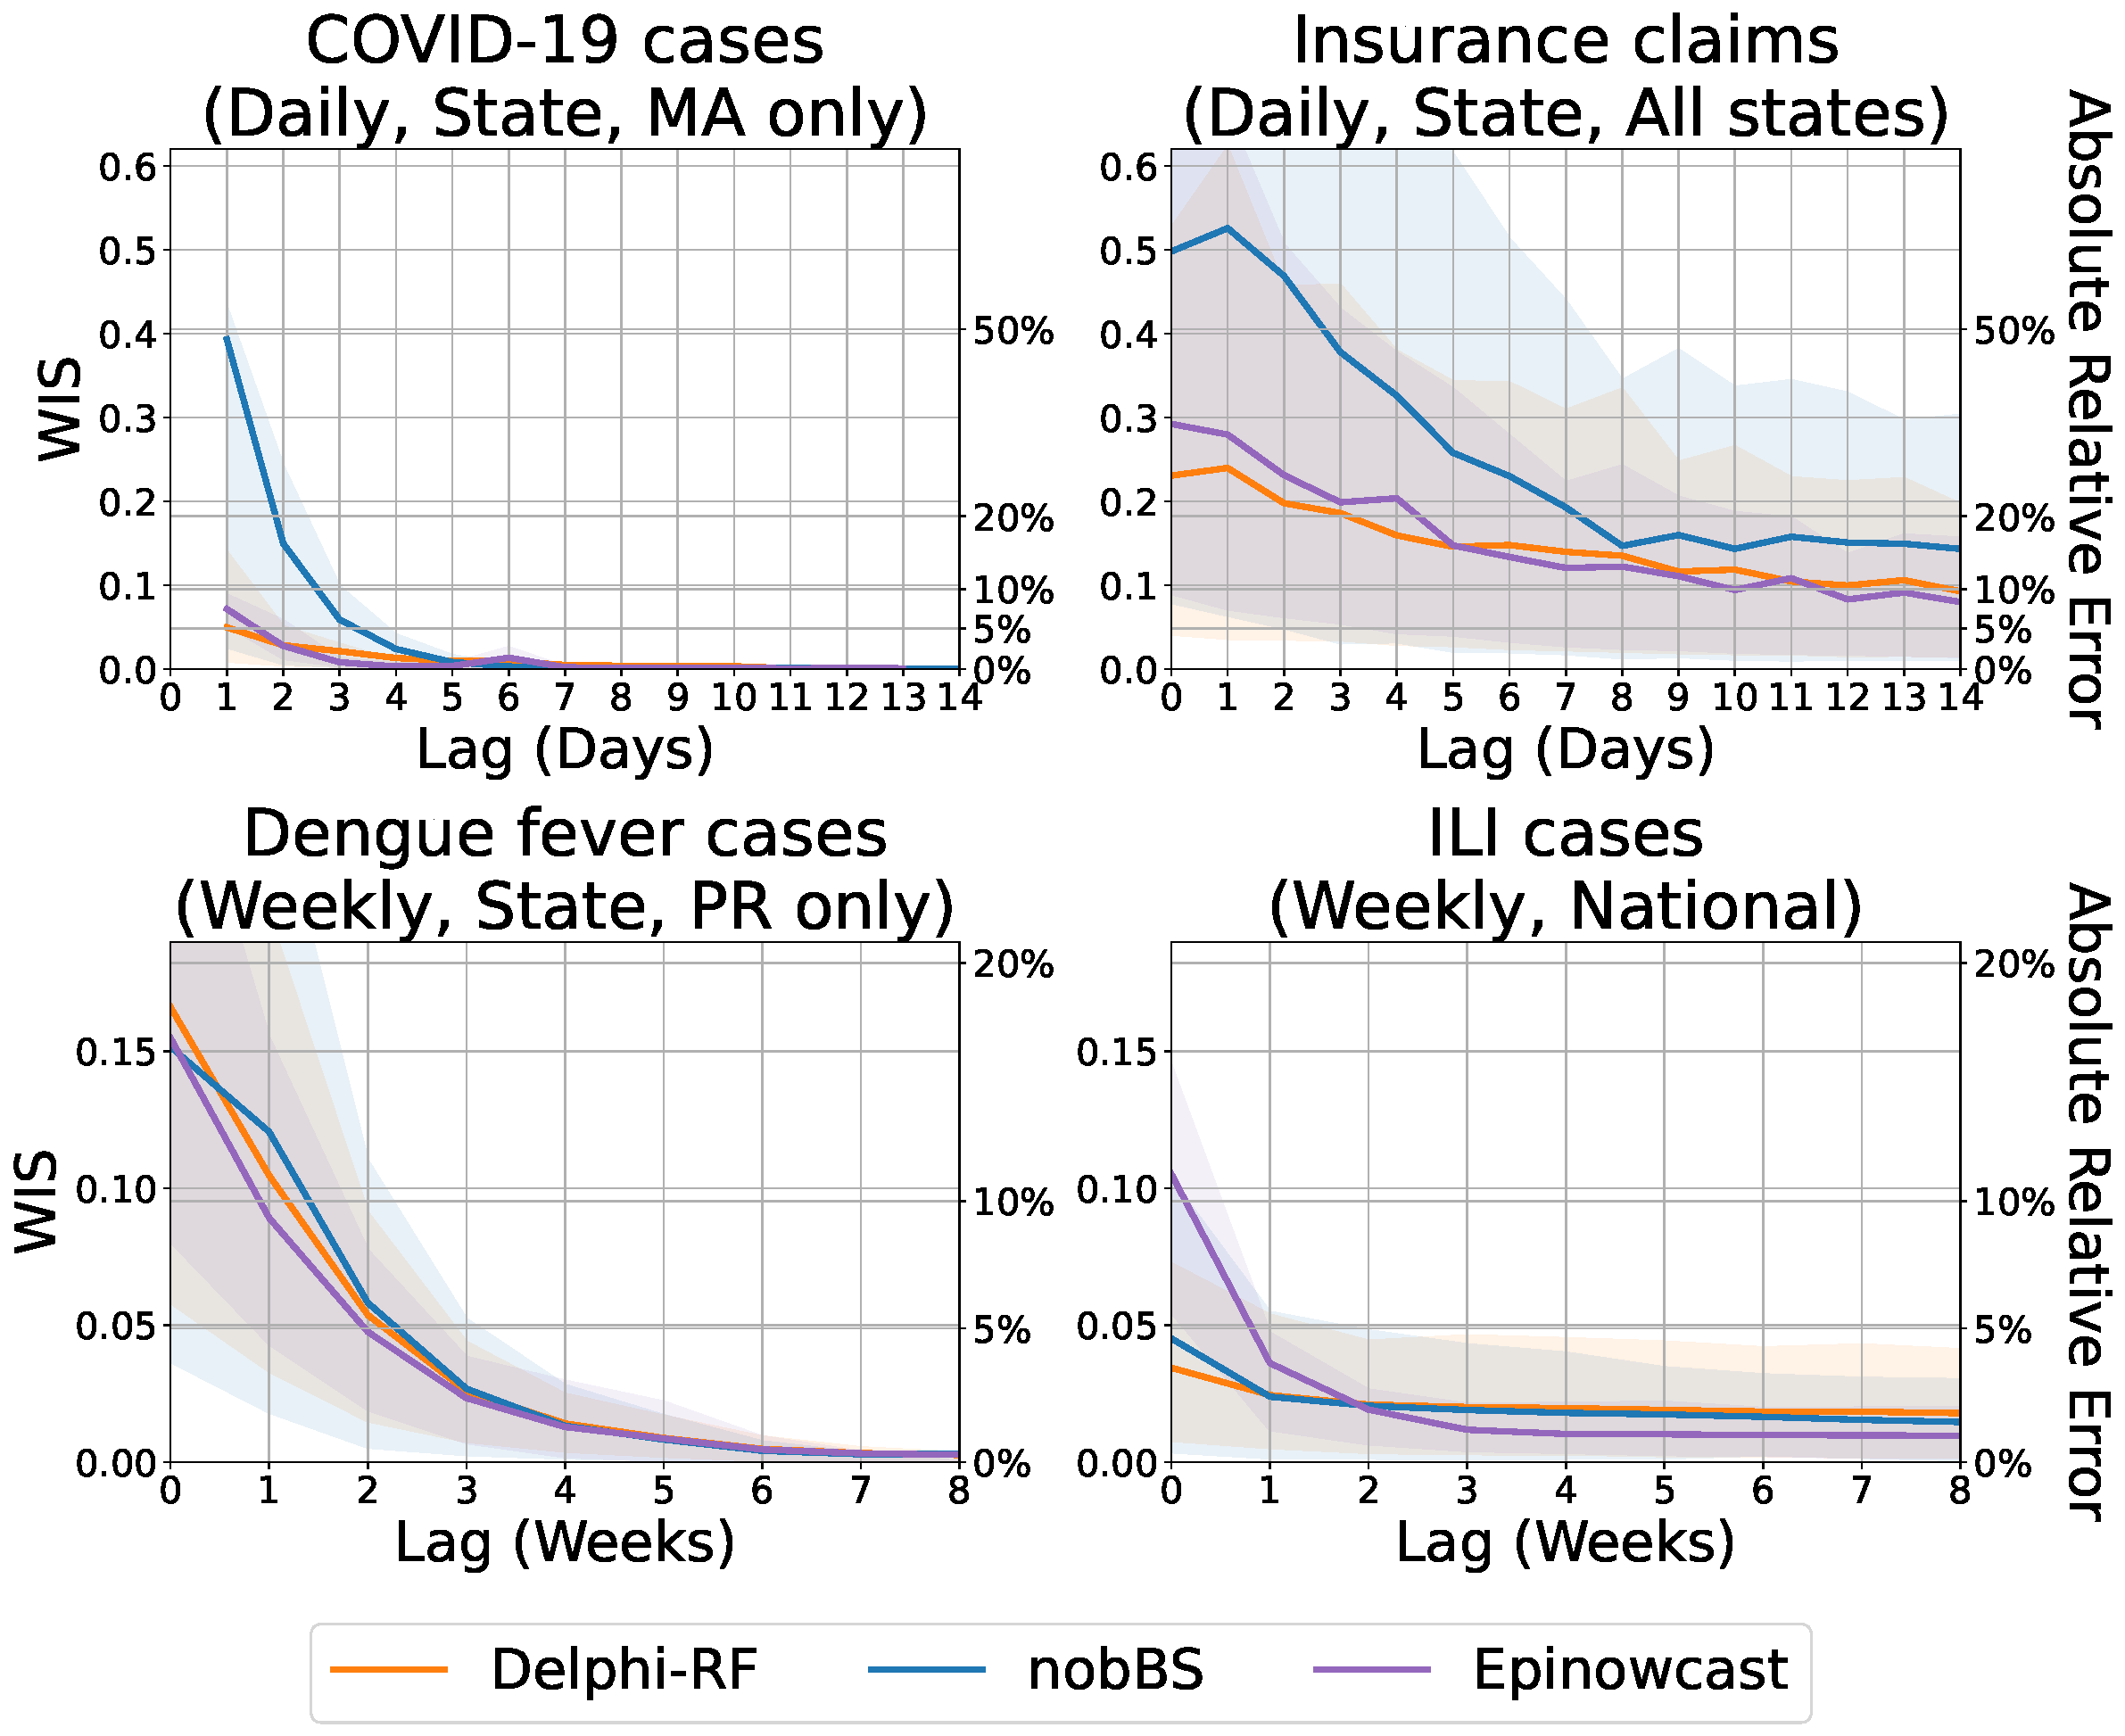
\includegraphics[width=\textwidth]{figs/experiment_count_result_evl_general_for_comparison.pdf}
   \caption{\emph{\textbf{Comparison of count forecast evaluation results with NobBS and Epinowcast.} Top: Forecasts of the number of finalized confirmed COVID-19 case counts in MA and forecasts of the number of insurance claims in all states based on CHNG outpatient insurance claims data. Bottom: Forecasts of the number of dengue fever cases in Puerto Rico and forecasts of the number of ILI case counts nationwide. Solid lines represent the mean WIS, which approximates absolute relative errors between the most recent report and the target, averaged over locations and reference dates for each lag. Shaded areas indicate the 10th to 90th percentile interval.}}

\end{figure}

All experiments were conducted on an Apple Mac Mini equipped with a 3.0 GHz 6-core Intel Core i5 processor, running R version 4.4.2.

\begin{table}[h!]
\centering
\resizebox{\textwidth}{!}{%

\begin{tabular}{cc|cccc}
\hline
\multicolumn{2}{c|}{\multirow{2}{*}{\makecell{\textbf{Computing Time(s)}\\\makecell{(per location\\per report date)\\}}}} 
& \multicolumn{4}{c}{\textbf{Model}} \\
\multicolumn{2}{c|}{} 
& \makecell{Delphi-RF\\Training\\(once/week or month)} 
& \makecell{Delphi-RF\\Testing} 
& \makecell{Epinowcast} 
& \makecell{NobBS} \\
\hline
\multirow{6}{*}{\rotatebox{90}{\textbf{Dataset}}} &\makecell{Confirmed Cases\\(Daily, State, MA only)} & $6.773 \pm 0.018$ &$0.369\pm 0.006$  &$406.097\pm 16.190$ &$24.220\pm 0.675$ \\
&\makecell{Insurance Claims \\ (Daily, State, All states)}   & $23.712\pm 0.029$ &$0.819\pm 0.008$&$2386.512 \pm 230.895$ &$96.012 \pm  0.453$ \\
 
% &\makecell{Insurance Claims\\(Weekly, State)} &$0.408 \pm 0.001$ &$0.003\pm 0.000$ &$10.332 \pm 0.129$ &$1.638 \pm 0.002$ \\ 
 &\makecell{Dengue Fever Cases\\(Weekly, State, PR only)} &$6.848 \pm 0.106$ &$0.153\pm 0.008$  &$64.628 \pm 0.395$ &$8.337\pm 0.033$ \\
 &\makecell{ILI Cases\\(Weekly, National)} &$2.006 \pm  0.032$ &$0.136\pm 0.003$  &$18.373 \pm 2.139$ &$5.960\pm 0.055$ \\
 \hline
\end{tabular}
}
\caption{\emph{\textbf{Computing time comparison across methods and datasets.} 
Computing time required by different methods applied to various datasets, measured per location and per report date. 
The table presents the mean and standard error of the mean (SEM) for computing time. For daily data, all models are trained and generate forecasts every 30 days for CHNG outpatient insurance claims and every 7 days for MA-DPH COVID-19 confirmed cases. For weekly data, models are trained and generate forecasts on a weekly basis. To ensure a fair comparison, all settings—including maximum delay and training window size—are kept the same across methods.}}

\label{tab:full-width}
\end{table}

As shown in Figure 8, our model delivers accurate forecasts across all evaluated datasets. For daily COVID-19 signals, Delphi-RF consistently outperforms NobBS and achieves accuracy comparable to that of Epinowcast. To ensure a fair comparison across methods, a fixed 180-day training window is used—a conservative choice made to accommodate the computational demands of more resource-intensive methods such as Epinowcast. This restriction, however, can be suboptimal for Delphi-RF. In fact, forecast accuracy improves for certain reference dates and locations when the training window is extended (e.g., FL and NJ in Figures S10 and S32, Appendix C), with only a modest increase in computation time. For example, increasing the window to 365 days results in less than a twofold increase in runtime for both the Insurance Claims and MA-DPH COVID-19 case data (Table 2, Appendix B). In contrast, Epinowcast and NobBS become computationally infeasible under the same setting, with Epinowcast exceeding the 30-minute runtime cutoff for a single location–report-date pair. When applied to Insurance Claims data across all 50 states, sequential training using either method with a 180-day or longer window would require more than two days—rendering them impractical for daily forecasting tasks.

For weekly data, Delphi-RF exhibits competitive forecasting performance for dengue fever cases in Puerto Rico. In the case of national ILI counts, Delphi-RF outperforms both benchmark methods at lag 0. Although Delphi-RF does not outperform Epinowcast when the reporting lag exceeds 3 weeks, the absolute relative errors for all methods are sufficiently low—consistently below 2.5\%—rendering performance differences practically negligible.

The runtime reported in Table 1 reflects both the training and testing phases required by our model (including the computing time for data pre-processing), which is substantially faster than the other two methods. Unlike Epinowcast and NobBS, which require simultaneous training and forecasting, our model benefits from the modularity of machine learning frameworks, allowing for independent training and inference. Once trained, the model can be repeatedly applied to generate forecasts for new data. This flexibility allows users to tailor the training frequency to operational constraints, a feature not available in Epinowcast or NobBS. The efficiency also enables our model to produce revision forecasts for multiple signals at different temporal resolutions in real time while requiring significantly fewer computational resources. 









\section{Conclusion and Discussion}
This paper introduces a comprehensive framework designed for modeling data revision patterns and generating distributional projections for the revised variables of interest. The versatility of the proposed framework is noteworthy, as it is applicable to a spectrum of data revision challenges where the sequences of data revisions are both available and sufficiently smooth. The application of our model extends across diverse public health data sources, encompassing CHNG outpatient COVID claims data, Quidel COVID Antigen test data, and confirmed cases data from MA DPH. 

To reiterate, we purposely defined our target of projection to be the quantities of interest reported after a certain number of days (target lag) as opposed to awaiting the eventual finalized version, a process that often unfolds several months later for numerous public health data sources. The metric employed for assessing projection performance is based on the target values, assumed to be sufficiently proximate to the finalized values, rather than relying on the actual finalized values. As expounded in the preliminary section, we consciously opt for a trade-off, sacrificing a degree of accuracy relative to the finalized values in favor of a more expeditious response to pattern changes.

Concerning our evaluation approach, we have embraced a symmetrical perspective to gauge relative errors, wherein we assess the absolute deviation between the log-scale predictions and the actual values. This evaluation methodology is scale-independent, ensuring that it remains unaffected by the magnitude of the values under comparison. This characteristic proves particularly advantageous given the wide range of epidemic quantities across different reference dates and locations. Notably, when the original value approaches zero, the relative error can escalate significantly, introducing sensitivity issues. It is imperative to acknowledge that our chosen method inherently grapples with challenges associated with the application of relative errors, as illustrated in Figure X, where suboptimal projection performance is observed for locations naturally characterized by small target fractions.

our framework excels in delivering precise and timely projections for the target version of epidemic quantities of interest. These projections serve a dual purpose by not only alerting surveillance systems to abrupt changes in data revision patterns but also proving instrumental in epidemic forecasting. The ability to preemptively correct both predictors and responses in forecasting challenges can contribute to timely and accurate forecasts in the realm of epidemic monitoring and response.



 

%% TODO: Not the latest version.  
%% Use log 10 or natural log scale? natural log add the second axis? 
\begin{figure}
    \centering
    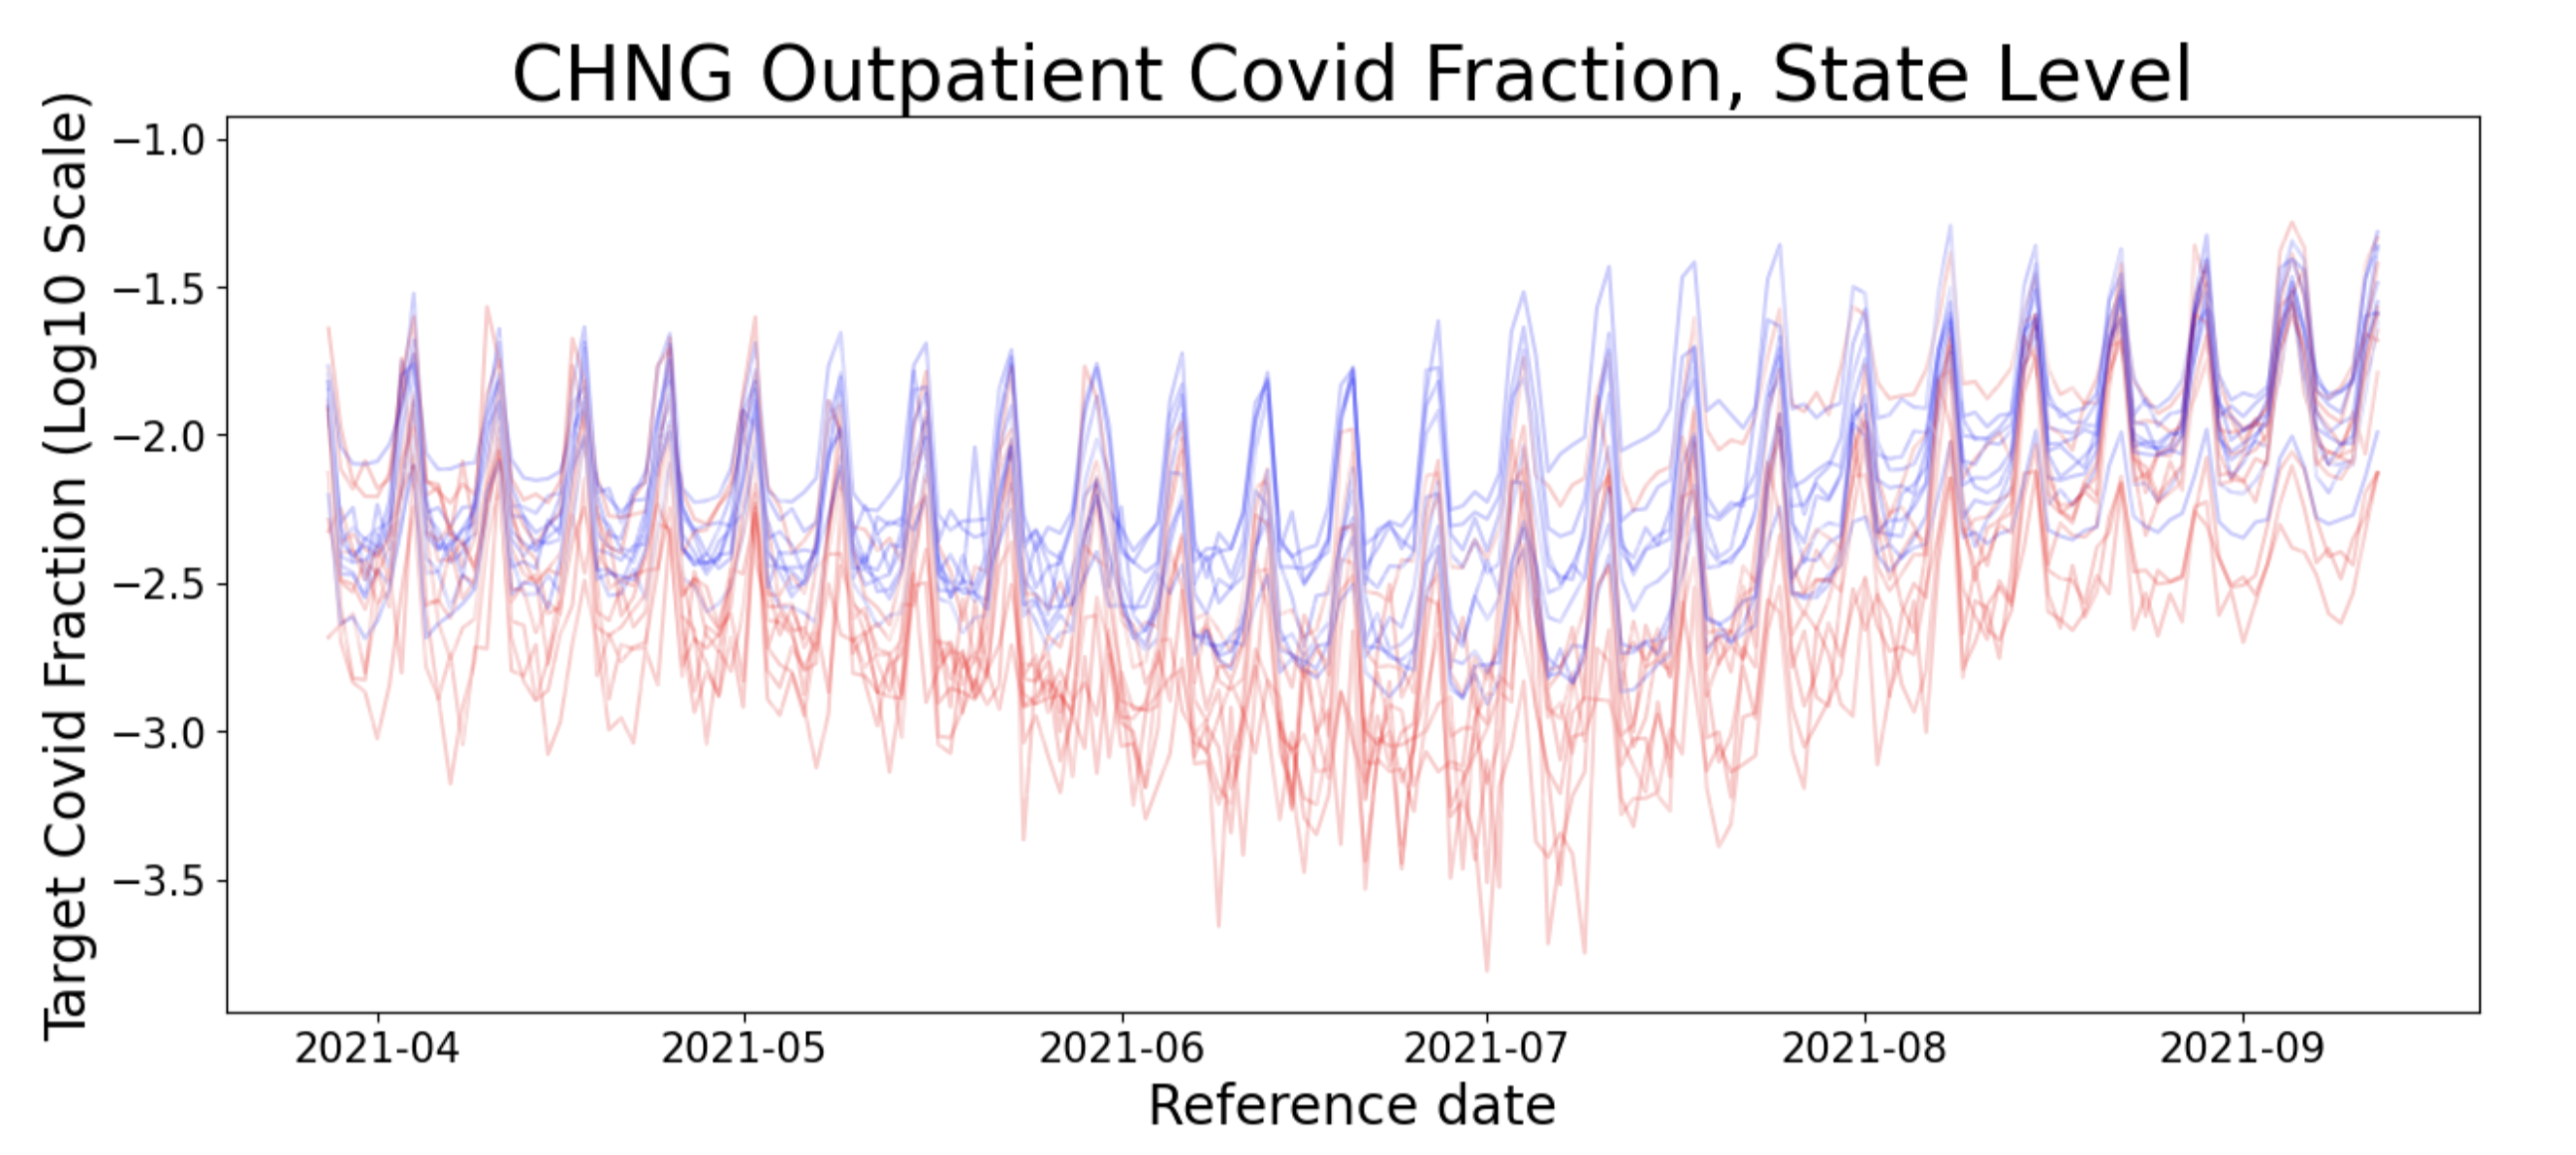
\includegraphics[width=\textwidth]{figs/evl_comparison_states.png}
    \caption{\textit{red lines represent the 10 states with the worst prediction performance while blue lines represent the 10 states with the best prediction performance}}
\end{figure}

%Due to the exponential nature, situations in which models missed the %beginning of upswings are more strongly emphasized while failing to %predict a downturn following a peak is less severely penalized. 
\begin{figure}
    \centering
    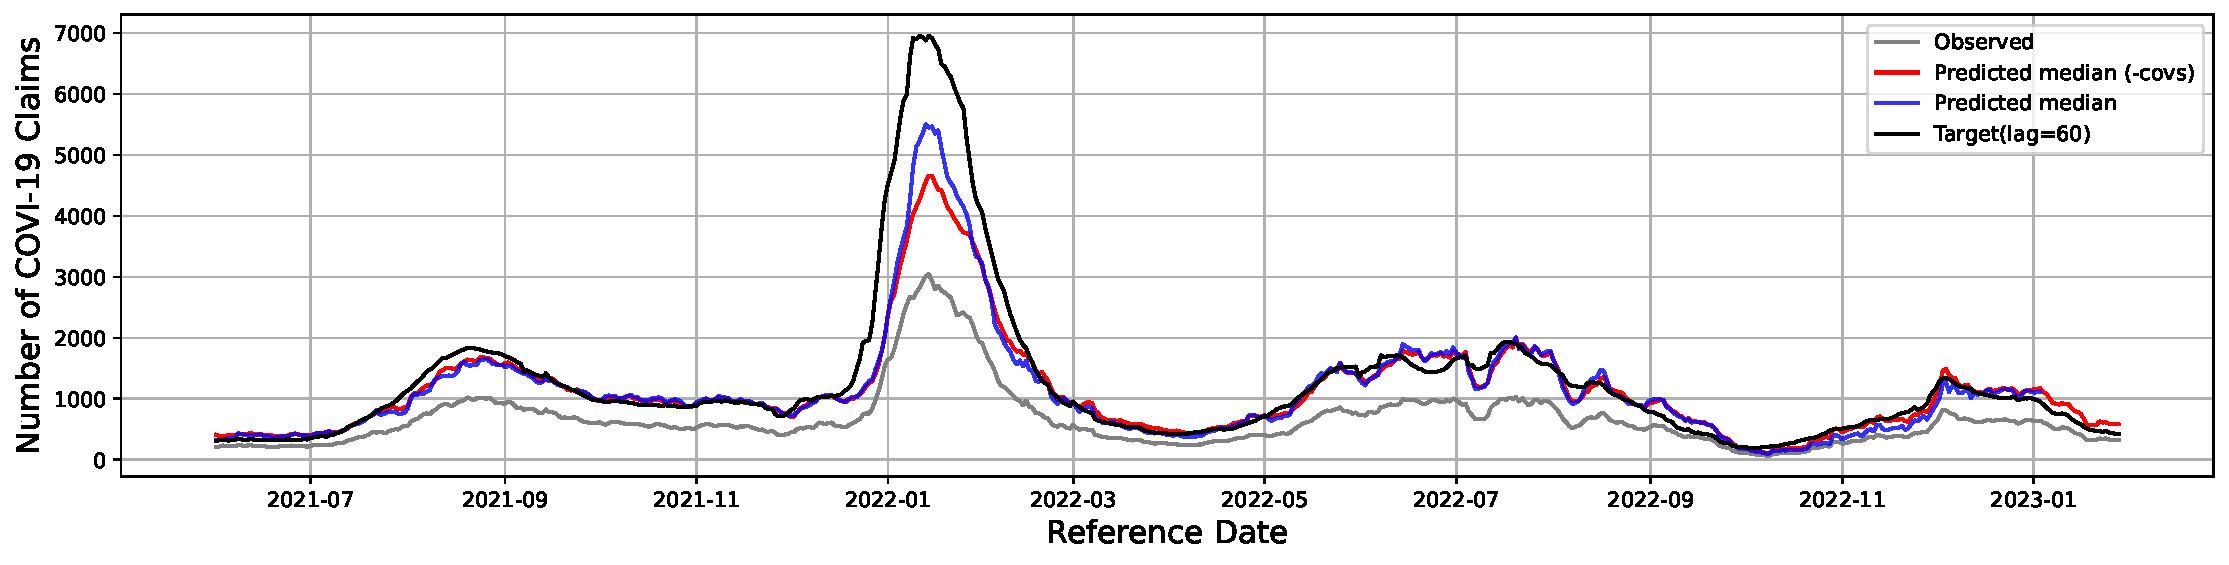
\includegraphics[width=\textwidth]{figs/pred_problem_in_ca.pdf}
    \caption{\textit{the backfill correction}}
\end{figure}

\begin{figure}
    \centering
    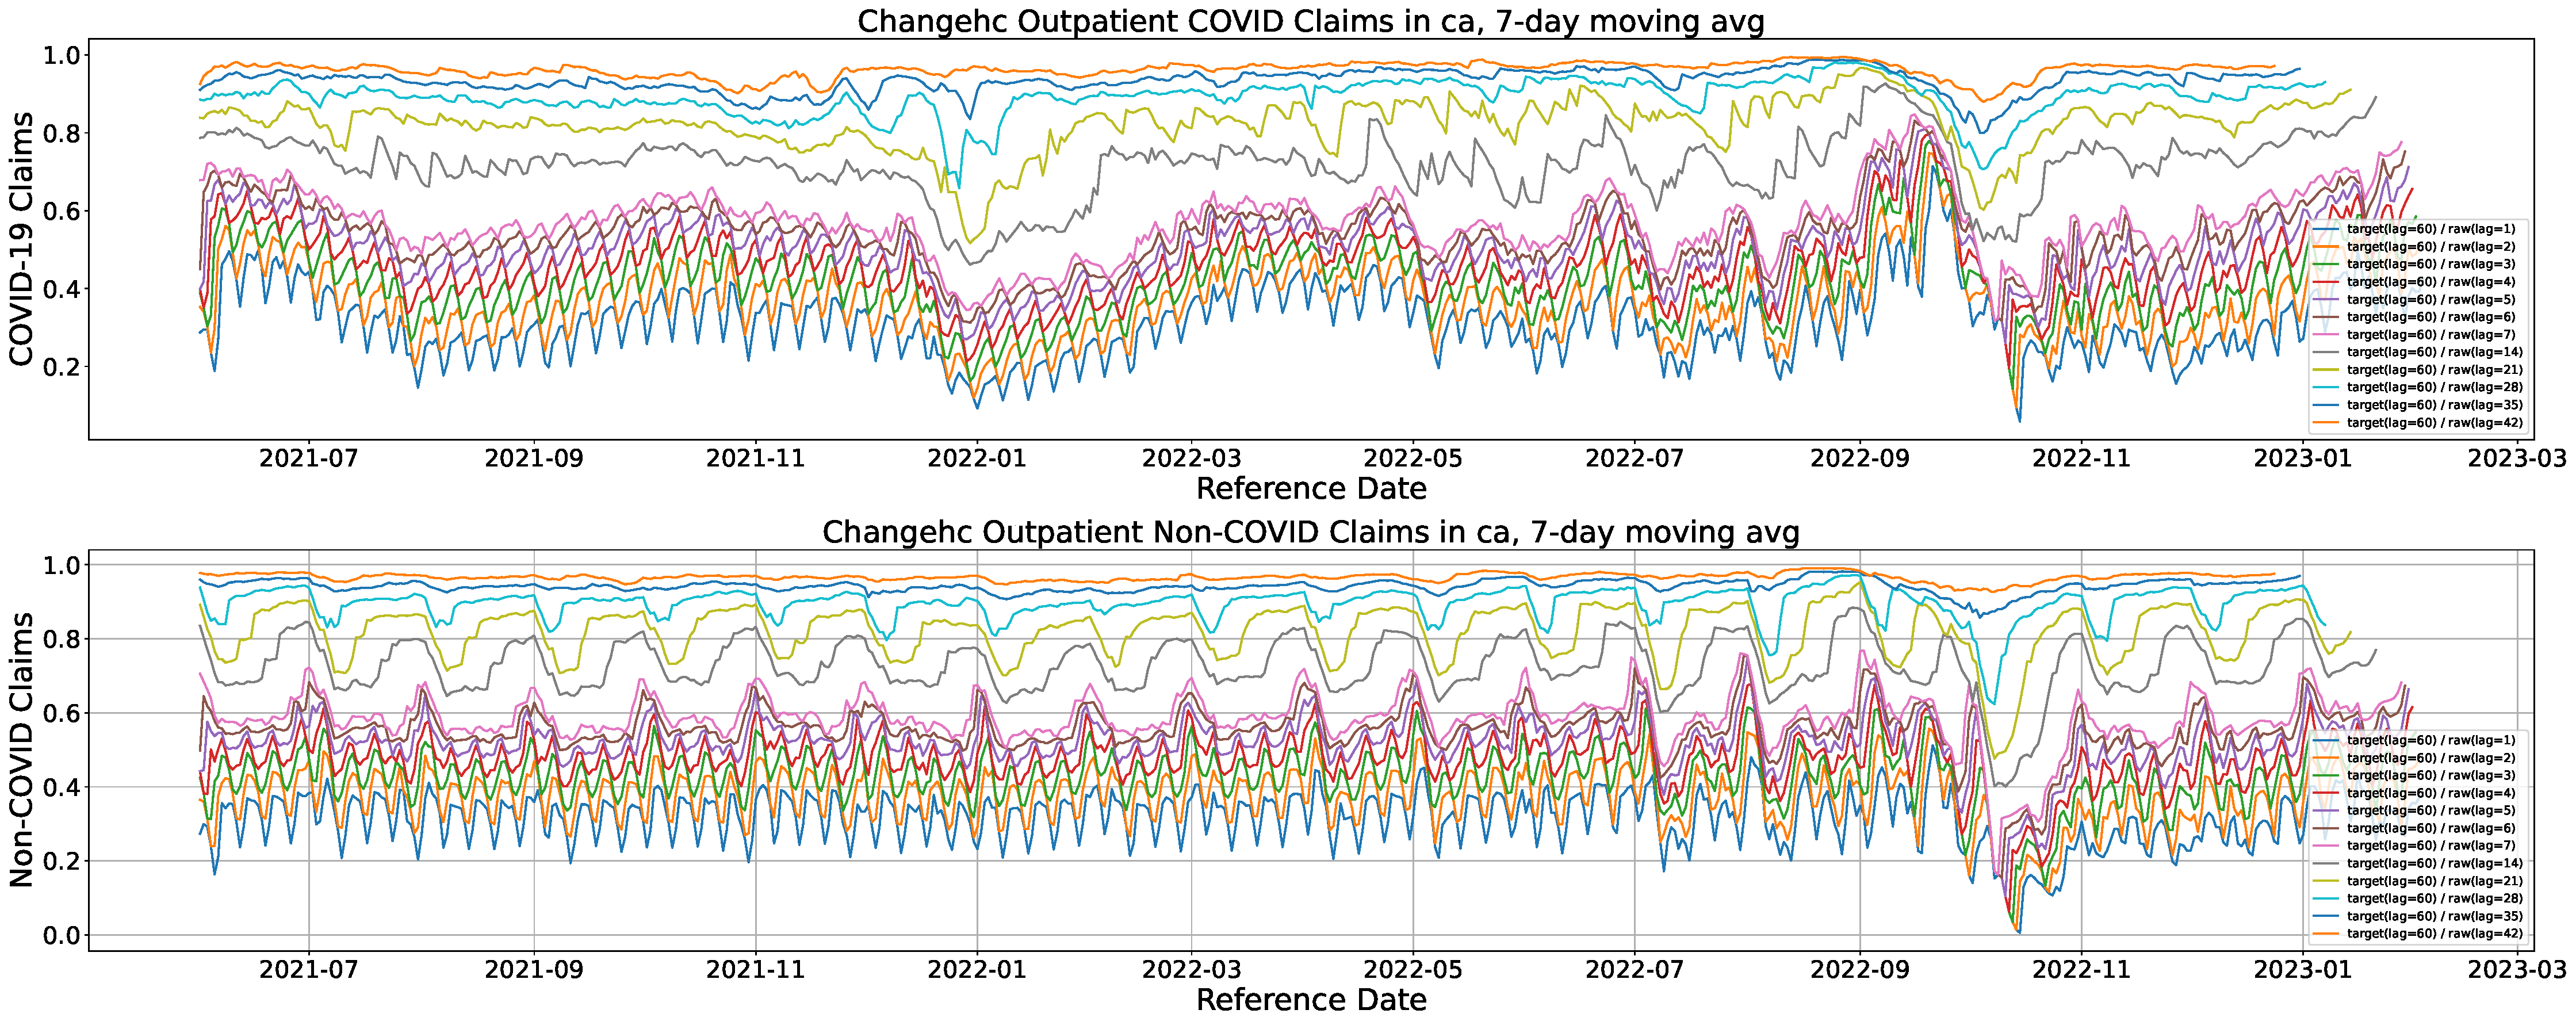
\includegraphics[width=\textwidth]{figs/new_covs_zoom_in.pdf}
    \caption{\textit{the backfill correction}}
\end{figure}




\section{Acknowledgements}
The authors are grateful to Ryan Tibshirani, Logan Brooks, Will Townes for insightful conversations. 
This work was supported by a fellowship from the Center for Machine Learning and Health at Carnegie Mellon University, and by ...


\clearpage

% TODO at the end
% Either type in your references using
% \begin{thebibliography}{}
% \bibitem{}
% Text
% \end{thebibliography}
%
% or
%
% Compile your BiBTeX database using our plos2015.bst
% style file and paste the contents of your .bbl file
% here. See http://journals.plos.org/plosone/s/latex for 
% step-by-step instructions.
% 
\bibliographystyle{plos2015} % Specify the bibliography style
\bibliography{bib} % Include the bibliography file


\clearpage
\appendix

\section{Example of Revision Behavior and Target Lag Selection}
\renewcommand{\thefigure}{S\arabic{figure}} % Changes the figure numbering to S1, S2, etc.
\setcounter{figure}{0} % Resets the figure counter
\begin{figure}[h!]
    \centering
    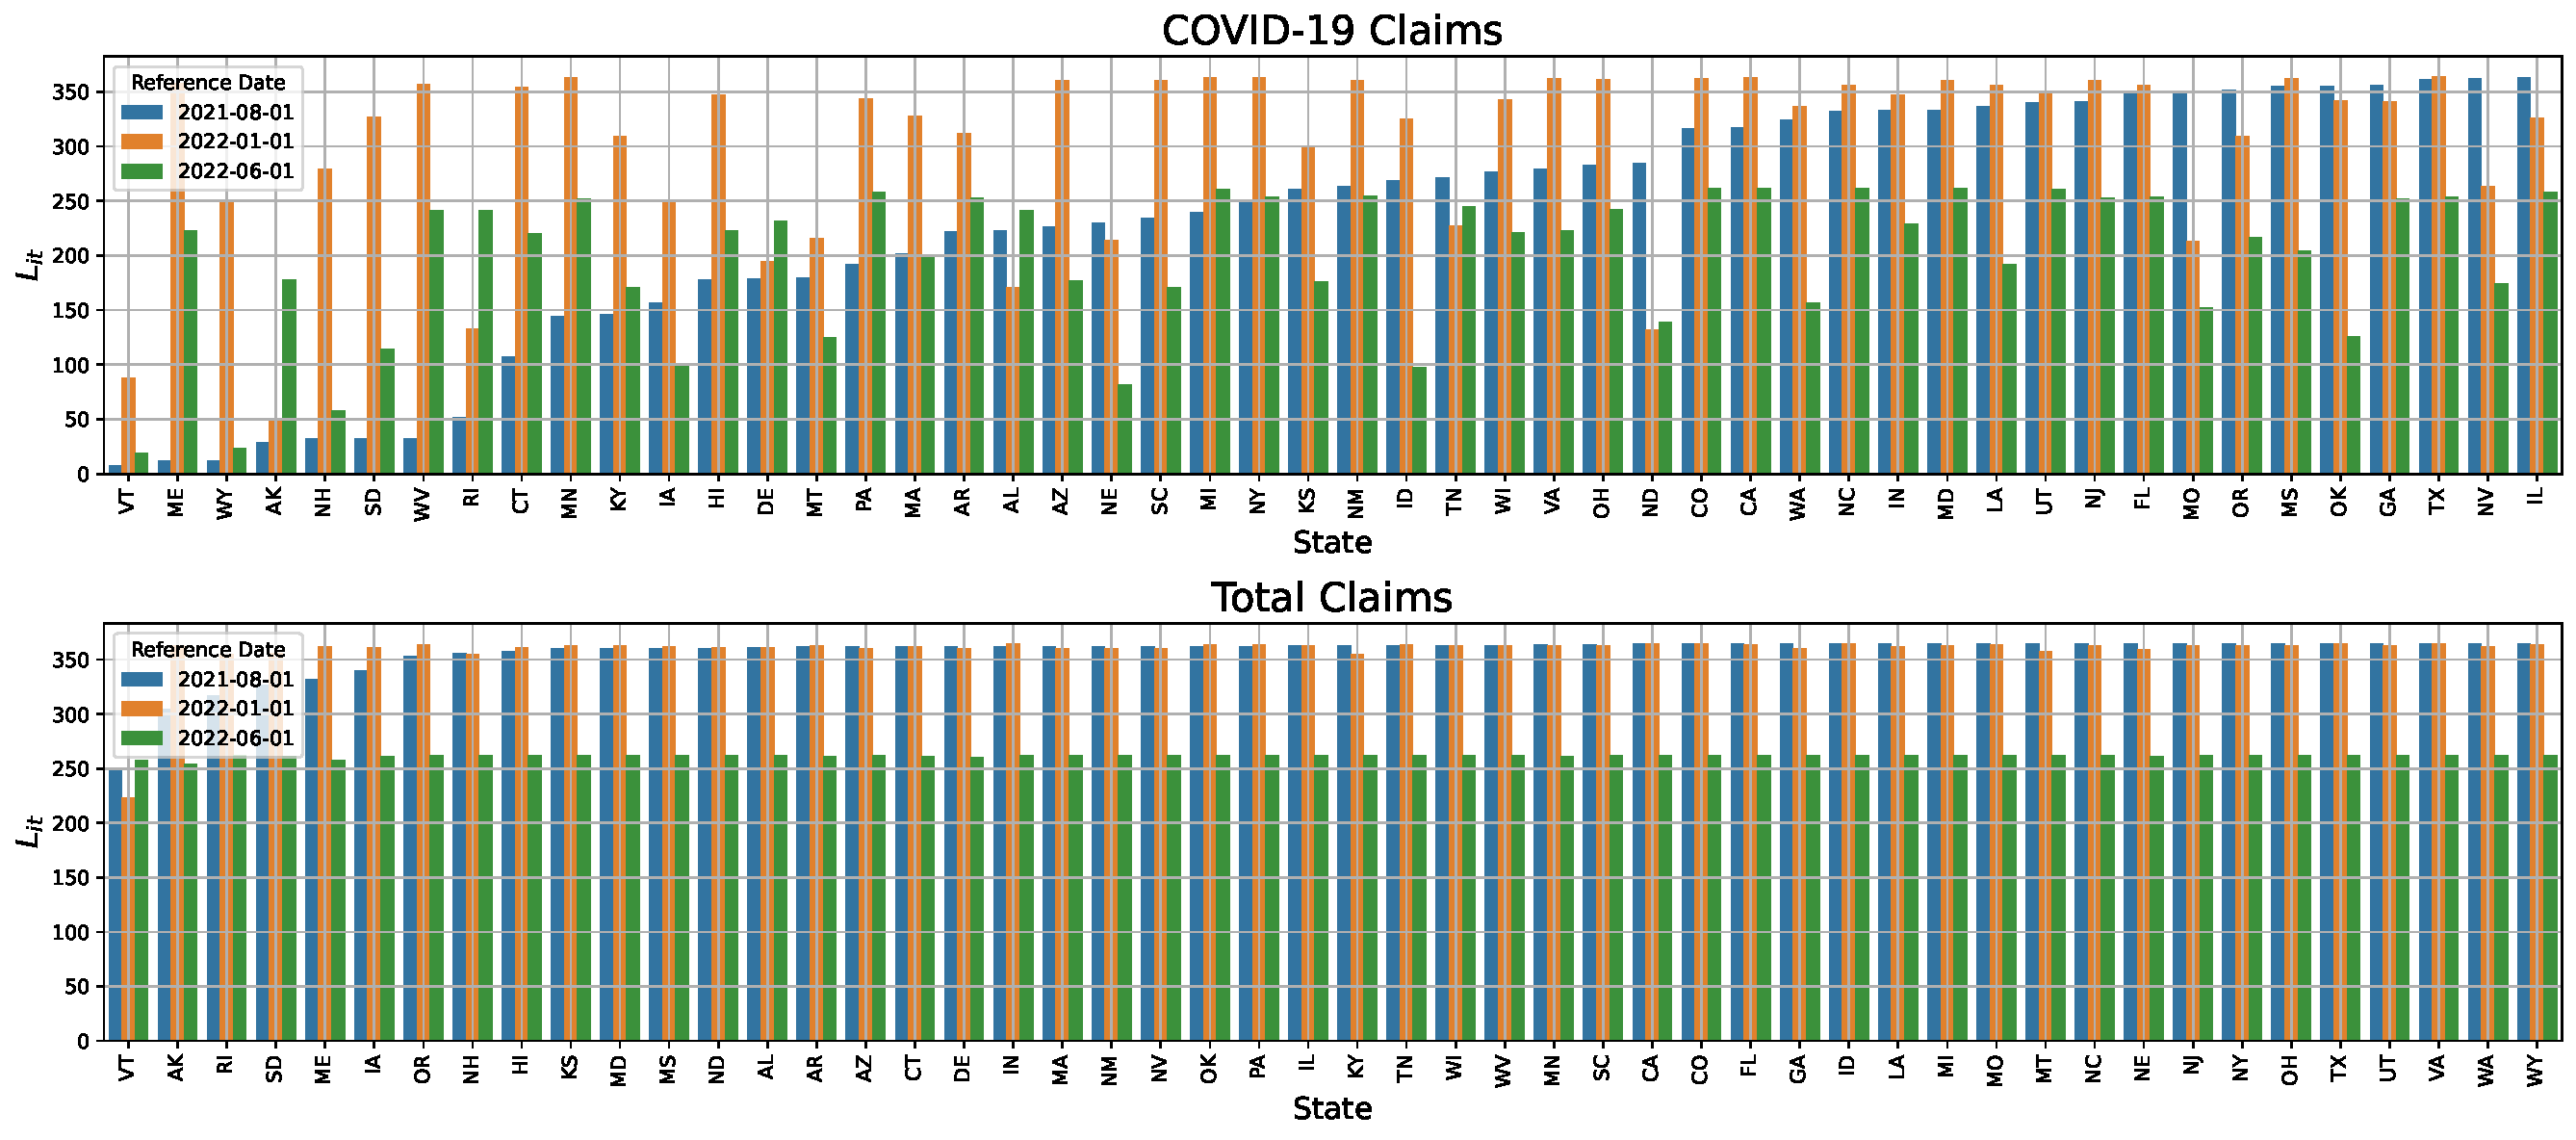
\includegraphics[width=\textwidth]{figs/Lit_examples.pdf}
    \caption{\emph{\textbf{Lag convergence patterns across states.} Top: Comparison of the lags required for convergence across states, shown for a sample of different reference dates based on CHNG outpatient COVID-19 insurance claims. Bottom: Same as the top panel, but based on CHNG outpatient total insurance claims data.}}

\end{figure}


\section{Computational Cost of Training Window Variation for Daily Data}

\begin{table}[h!]
\centering
\resizebox{\textwidth}{!}{%
\begin{tabular}{|c|c|c|c|c|}
\hline
\multicolumn{2}{|c|}{\textbf{Computing Time (s)} (per location per report date)} 
& \multicolumn{3}{c|}{\textbf{Model}} \\
\hline
\makecell{\textbf{Training Window}\\\textbf{(days)}} & \textbf{Data} 
& \makecell{Delphi-RF\\Training\\(once/week or month)} 
& \makecell{Epinowcast} 
& \makecell{NobBS} \\
\hline
\multirow{2}{*}{180} 
& \makecell{Confirmed Cases\\(Daily, State, MA only)} & $6.773 \pm 0.018$   &$406.097\pm 16.190$ &$24.220\pm 0.675$ \\
& \makecell{Insurance Claims\\(Daily, State, All states)} & $23.712\pm 0.029$ &$2386.512 \pm 230.895$ &$96.012 \pm  0.453$ \\
\hline
\multirow{2}{*}{365} 
& \makecell{Confirmed Cases\\(Daily, State, MA only)} & $7.348 \pm 0.024$  &$1289.363\pm 79.974$ &$59.549\pm 1.011$ \\
& \makecell{Insurance Claims\\(Daily, State, All states)} & $37.389\pm 0.042$ &- &$297.092 \pm 1.709$ \\ 
\hline
\end{tabular}

}
\caption{\emph{\textbf{Runtime comparison across methods for daily data at different training windows.}
This table presents the mean and standard error of the mean (SEM) for computing time (in seconds) required by different forecasting methods, applied to daily COVID-19 datasets. Results are reported per reference date and location. Models are trained and used to generate forecasts every 30 days for CHNG insurance claims data and every 7 days for MA-DPH confirmed case data. The comparison is performed under two training window settings (180 and 365 days), with all other configurations held constant to ensure a fair evaluation of runtime differences across methods.}}
\label{tab:full-width}
\end{table}

\clearpage
\section{Complete Set of DelphiRF Revision Forecasts by Reference Date}

Figures S2–S51 present DelphiRF revision forecasts for CHNG-provided insurance claims data at lag 7 across all 50 U.S. states. The model is re-trained every 30 days using training windows of 180 and 365 days, respectively. The format follows that of Figures 5 and 6 in the main text.

\foreach \state in \statepdfs {
  \begin{figure}[H]
    \centering
    \includegraphics[width=0.85\textwidth]{figs/appendix_\state_experiment_result_Insurance_claims_time_series.pdf}
    \caption{\emph{Forecast Accuracy for \MakeUppercase{\state}.}}
    \label{fig:claims-\state}
  \end{figure}
}

\clearpage
\section{Annotated Trend Categories in Target Values Across States}


\begin{figure}[h!]
    \centering
    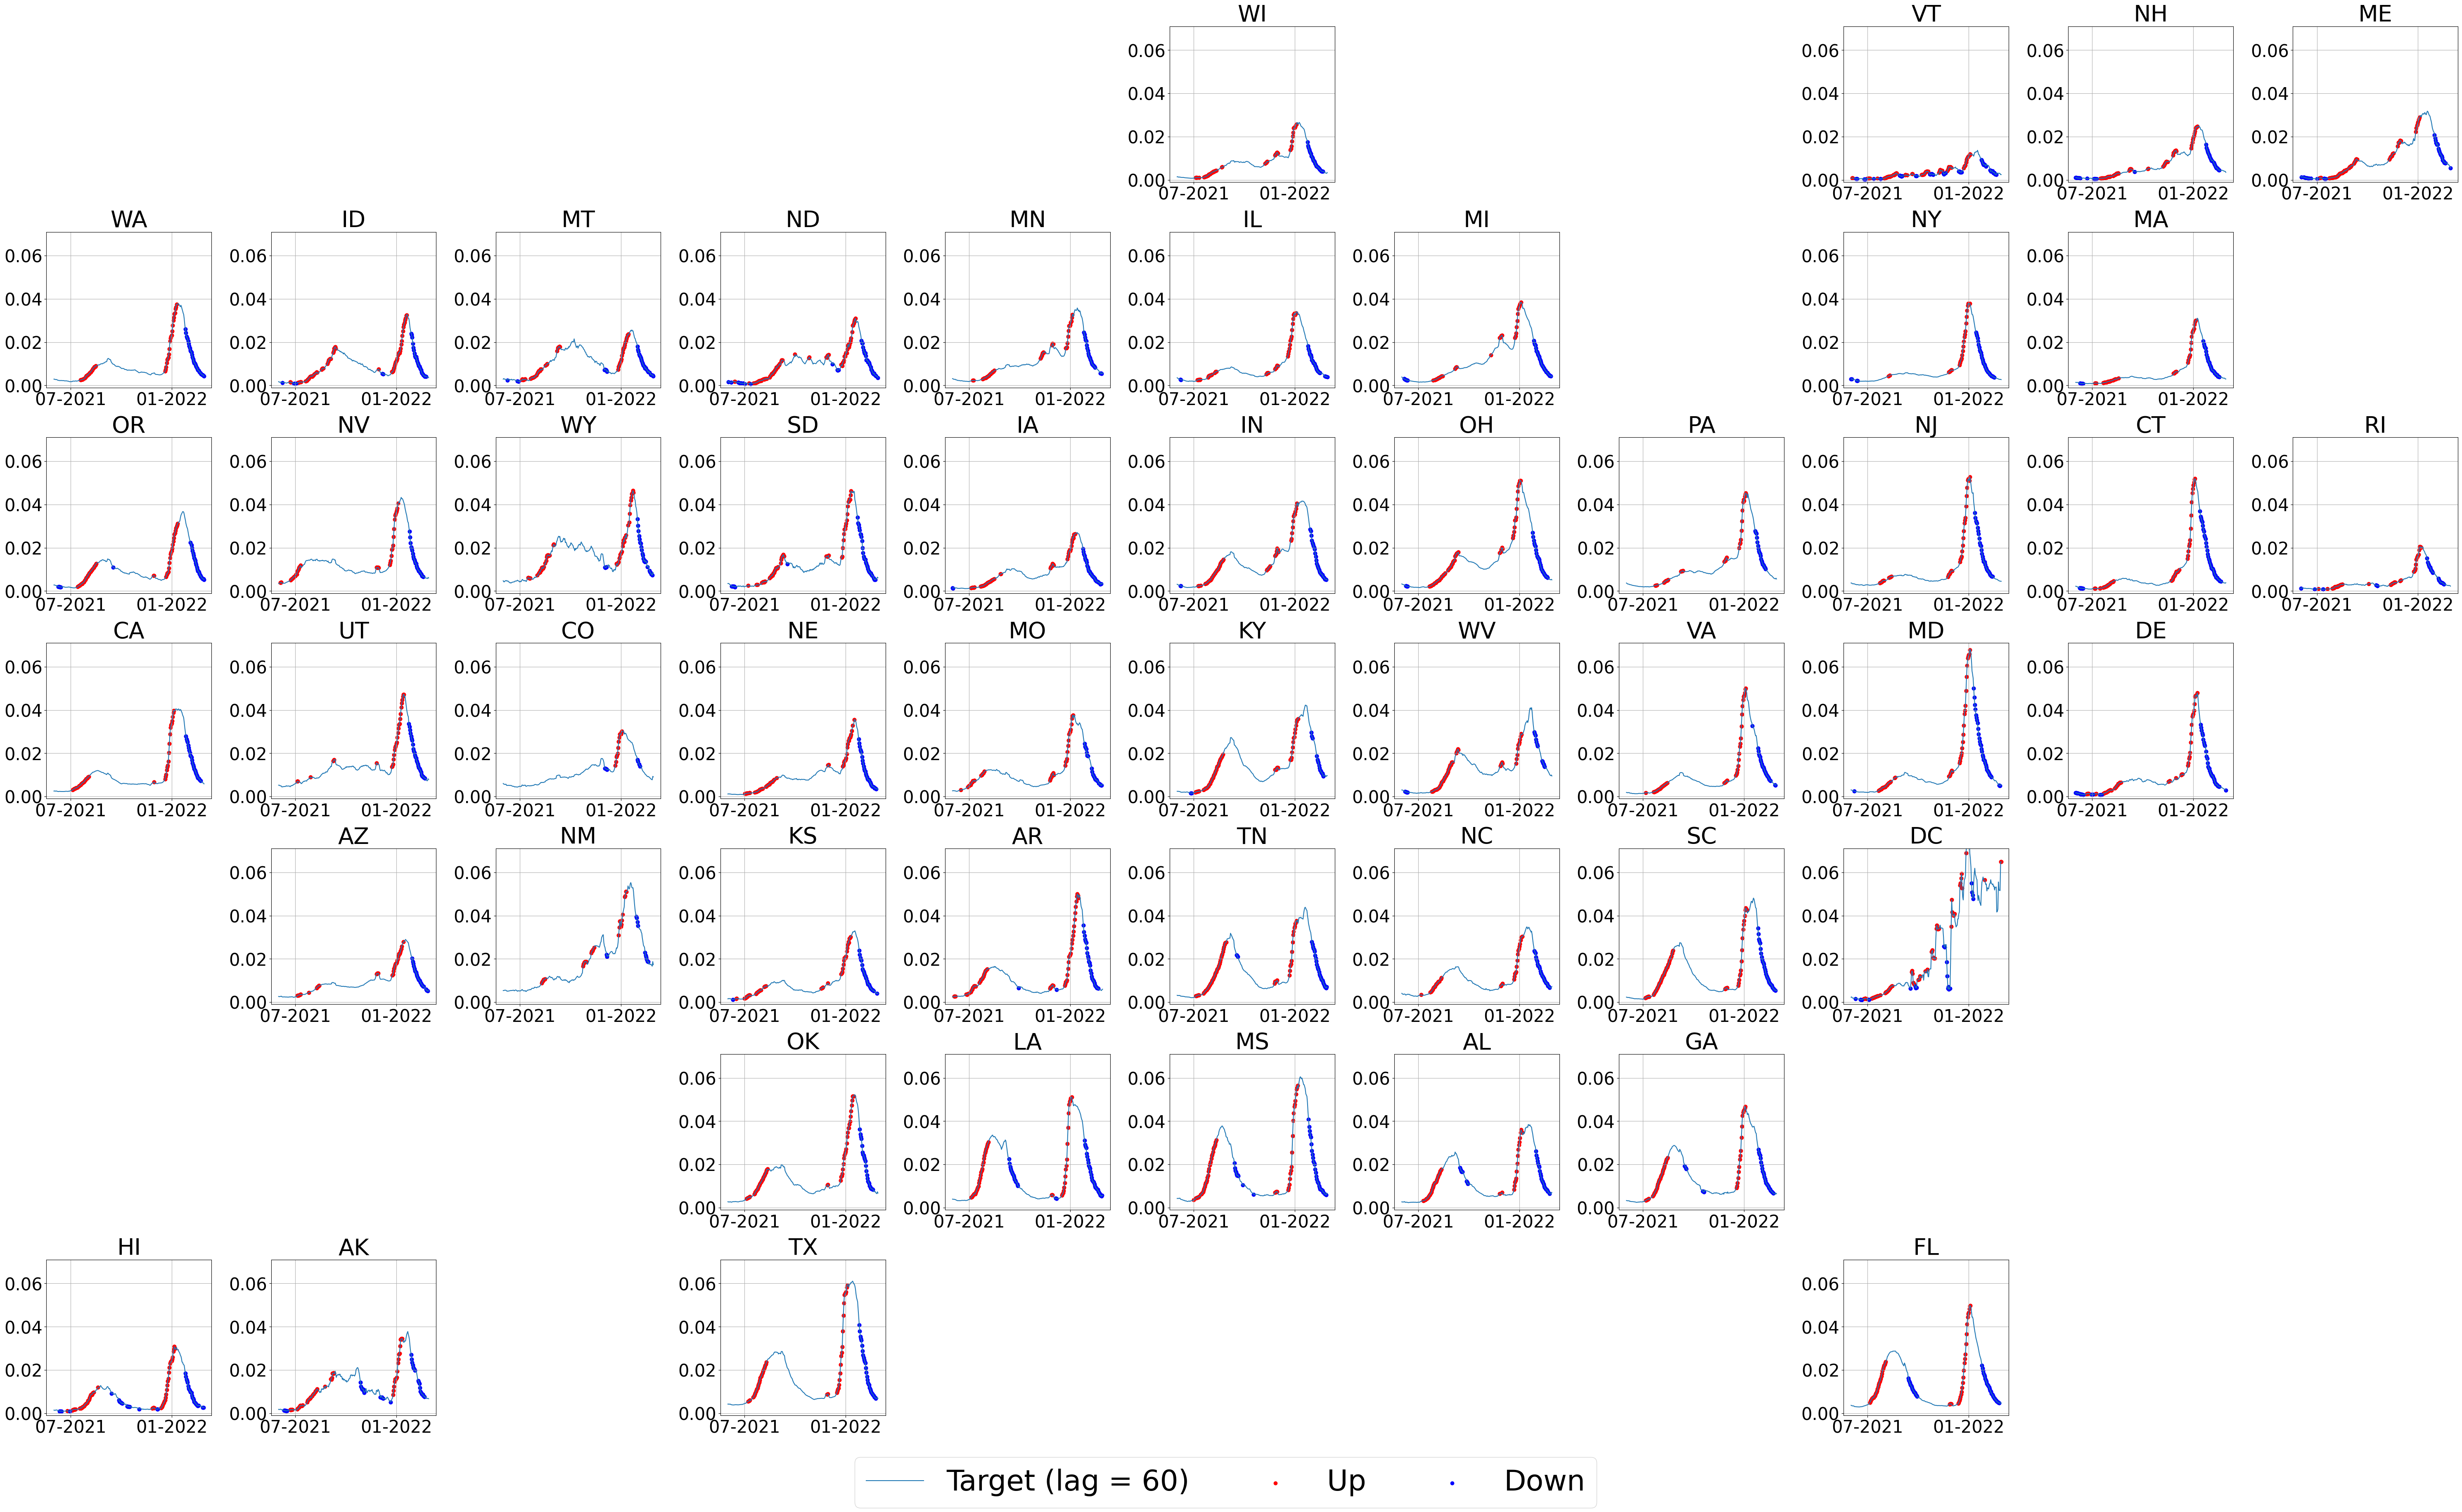
\includegraphics[width=\textwidth]{figs/temporal_annotation_for_states.png}
    \caption{\emph{Temporal Annotation of Trend Categories}}
\end{figure}


\nolinenumbers

\end{document}

